\documentclass[12pt,a4paper,titlepage,listof=totoc,bibliography=totoc,chapteratlists=0pt]{scrreprt}

\begin{filecontents*}{\jobname.xmpdata}
	\Keywords{VR, IOT, TODO}
	\Title{Unser tolles Thema -- wir sind suppa}
	\Author{Stefan Schwammal, Susi Schwammal}
\end{filecontents*}

\setcounter{tocdepth}{1}

\usepackage[utf8]{inputenc}
\usepackage[T1]{fontenc}
\usepackage{amsmath}
\usepackage{amsfonts}
\usepackage{amssymb}
\usepackage[table]{xcolor}
\usepackage{graphicx}
\usepackage[left=3.50cm, right=2.00cm, top=2.00cm, bottom=2.00cm,foot=1cm]{geometry}
\usepackage[splitrule,hang,flushmargin,multiple,bottom]{footmisc}
\usepackage{lmodern, textcomp}
\usepackage{lmodern}
\usepackage{pdfpages}
\usepackage[ngerman]{babel}
\usepackage{multicol}
\usepackage{subfig}
\usepackage{float}
\usepackage{array,tabularx,booktabs}
\usepackage{ragged2e}
\usepackage{lipsum}
\usepackage{wrapfig}
\usepackage{placeins}

\newcolumntype{M}[1]{>{\centering\arraybackslash}m{#1}}

\usepackage{enumitem}
\newlist{compactitem}{itemize}{3}
\setlist[compactitem,1]{label=\textbullet, nosep,leftmargin=1.5em,labelwidth=*,align=left}
\setlist[compactitem,2]{label=--, nosep,leftmargin=1.5em,labelwidth=*,align=left}
\setlist[compactitem,3]{label=\textopenbullet, nosep,leftmargin=1.5em,labelwidth=*,align=left}
\newlist{compactenum}{enumerate}{3}
\setlist[compactenum,1]{label=\arabic*., nosep,leftmargin=1.5em,labelwidth=*,align=left}
\setlist[compactenum,2]{label=\alph*., nosep,leftmargin=1.5em,labelwidth=*,align=left}
\setlist[compactenum,3]{label=\roman*., nosep,leftmargin=1.5em,labelwidth=*,align=left}
\newlist{compactdesc}{description}{3}
\setlist[compactdesc]{leftmargin=1.5em,labelwidth=*,align=left}

\usepackage{microtype}

\usepackage[parfill]{parskip}

\definecolor{bluekeywords}{rgb}{0.13,0.13,1}
\definecolor{greencomments}{rgb}{0,0.5,0}
\definecolor{redstrings}{rgb}{0.9,0,0}
\definecolor{lightgray}{gray}{0.9}
\definecolor{lightblue}{rgb}{0.93,0.95,1.0}

\usepackage{listings}

\makeatletter
\lstdefinestyle{lststyle}{
	basicstyle=%
	\ttfamily
	\lst@ifdisplaystyle\scriptsize\fi
}
\makeatother

\renewcommand{\lstlistlistingname}{List of Listings}
% TODO: define other languages as needed
\lstset{language=Python,
numbers=left,               
numberstyle=\tiny,          
showspaces=false,
showtabs=false,
breaklines=true,
lineskip=-1pt,
tabsize=2,
showstringspaces=false,
breakatwhitespace=true,
escapeinside={(*@}{@*)},
commentstyle=\color{greencomments},
keywordstyle=\color{bluekeywords}\bfseries,
stringstyle=\color{redstrings},
style=lststyle,
xleftmargin=17pt,
         framexleftmargin=17pt,
         framexrightmargin=5pt,
         framexbottommargin=4pt
}
\lstset{
morekeywords={base,var,in,out,dynamic,from,where,select,orderby,function,\$,group,by,into,yield,async,await,@,None,self,as,elif,with}
}
\lstdefinelanguage{TypeScript}{
	keywords={typeof, new, true, false, catch, function, return, null, switch, var, if, in, while, do, else, case, break, void, number, string, boolean, module, \$, export, for, this},
	keywordstyle=\color{blue}\bfseries,
	ndkeywords={class, export, boolean, throw, implements, import, this},
	ndkeywordstyle=\color{darkgray}\bfseries,
	identifierstyle=\color{black},
	sensitive=false,
	comment=[l]{//},
	morecomment=[s]{/*}{*/},
	commentstyle=\color{purple}\ttfamily,
	stringstyle=\color{red}\ttfamily,
	morestring=[b]',
	morestring=[b]"
}
\usepackage{caption}
\DeclareCaptionFont{white}{\color{white}}
\DeclareCaptionFormat{listing}{\colorbox[cmyk]{0.43, 0.35, 0.35,0.01}{\parbox{\textwidth}{\hspace{10pt}#1#2#3}}}
\captionsetup[lstlisting]{format=listing,labelfont=white,textfont=white} 
\captionsetup[table]{justification=centering, singlelinecheck=false}

\usepackage{setspace}
\newcommand{\MSonehalfspacing}{%
	\setstretch{1.44}%  default
	\ifcase \@ptsize \relax % 10pt
	\setstretch {1.448}%
	\or % 11pt
	\setstretch {1.399}%
	\or % 12pt
	\setstretch {1.433}%
	\fi
}

\newcommand{\setauthor}[1]{\ohead[]{#1}}

\usepackage[automark]{scrlayer-scrpage}
\pagestyle{scrheadings}
\automark{chapter}
\renewcommand\sectionmark[1]{\markright{\MakeMarkcase {\thesection\hskip .5em\relax#1}}}
\rohead{\ifnum\expandafter\pdfstrcmp\botmark=0 \rightmark\else\leftmark{} --- \rightmark\fi}
\ihead[]{\headmark}
\chead[]{}
\ohead{}
\cfoot[]{}
\ofoot[\pagemark]{\pagemark}
\setheadsepline{.1pt}

\usepackage[hyphens]{url}

\usepackage[a-1b]{pdfx}

\usepackage{hyperref}
\hypersetup{
    colorlinks=true,
    linkcolor=black,
    filecolor=magenta,
    urlcolor=cyan,
}

\usepackage[nonumberlist,toc,nopostdot]{glossaries}

\usepackage{chngcntr}
\counterwithout{footnote}{chapter}
\counterwithout{figure}{chapter}
\counterwithout{table}{chapter}
\AtBeginDocument{
	\counterwithout{lstlisting}{chapter}
	\urlstyle{sf}
}
\newcounter{RPages}

\makeatletter
\def\bstctlcite{\@ifnextchar[{\@bstctlcite}{\@bstctlcite[@auxout]}}
\def\@bstctlcite[#1]#2{\@bsphack
	\@for\@citeb:=#2\do{%
		\edef\@citeb{\expandafter\@firstofone\@citeb}%
		\if@filesw\immediate\write\csname #1\endcsname{\string\citation{\@citeb}}\fi}%
	\@esphack}
\makeatother

\clubpenalty=10000
\widowpenalty=10000
\displaywidowpenalty=10000
\interfootnotelinepenalty=10000

\title{AberGymMobile}
\author{Antonio Peric, Antonio Kuvac}

\makeindex
\makeglossaries
\begin{document}
\bstctlcite{IEEEexample:BSTcontrol}
\newcommand{\reminder}[1]
{ \textcolor{red}{<[{\bf\marginpar{\mbox{$<==$}} #1 }]>} }
\newcommand{\icode}[1]{\lstinline$#1$}
%\urlstyle{same}
%\setstretch{1.5}
\setstretch {1.433}
\renewcommand{\arraystretch}{1.2}

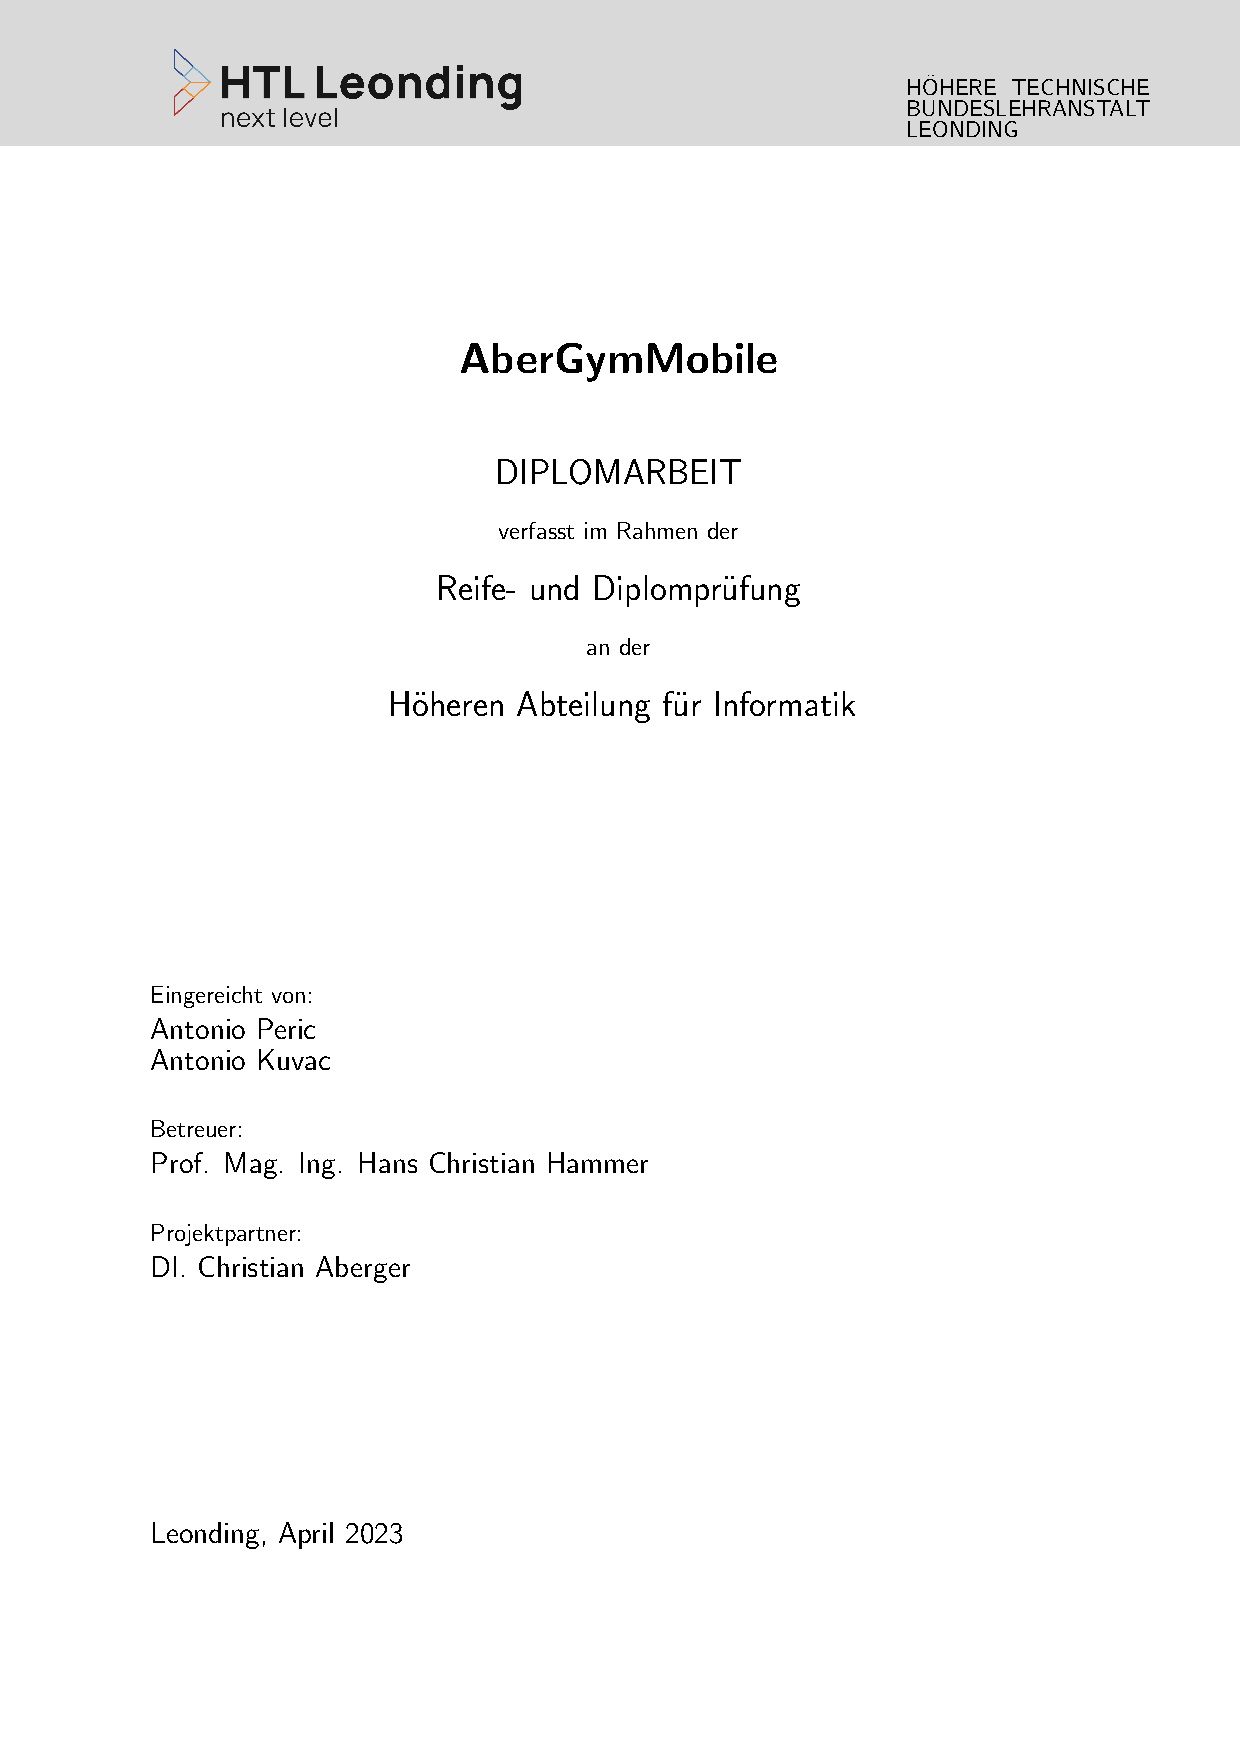
\includepdf{./titlepage/coversheet}
\pagenumbering{Roman}
\newpage
\thispagestyle{empty}
\vspace{3cm}
~ \\ \\
Ich erkläre an Eides statt, dass ich die vorliegende Diplomarbeit selbstständig und ohne fremde Hilfe verfasst, andere als die angegebenen Quellen und Hilfsmittel nicht benutzt bzw. die wörtlich oder sinngemäß entnommenen Stellen als solche kenntlich gemacht habe.

Die Arbeit wurde bisher in gleicher oder ähnlicher Weise keiner anderen Prüfungsbehörde vorgelegt und auch noch nicht veröffentlicht.

Die vorliegende Diplomarbeit ist mit dem elektronisch übermittelten Textdokument identisch.
\vspace{3cm}
% Hier kommt die Unterschrift drüber
\begin{tabbing}
Leonding, April 2022 \hspace{5cm} S. Schwammal \& S. Schwammal
\end{tabbing}
\vspace{10cm}
\newpage
\setcounter{page}{1}

\begin{spacing}{1}
    \chapter*{Abstract}
\end{spacing}
\begin{wrapfigure}{r}{0.3\textwidth}
    \begin{center}
      
\includegraphics[width=0.2\textwidth]{pics/question_mark.png}
    \end{center}
\end{wrapfigure}
Brief summary of our amazing work. In English.
This is the only time we have to include a picture within the text.
The picture should somehow represent your thesis.
This is untypical for scientific work but required by the powers that are.
\lipsum[6]
\newpage
\begin{spacing}{1}
    \chapter*{Zusammenfassung}
\end{spacing}
\begin{wrapfigure}{r}{0.3\textwidth}
    \begin{center}
      
\includegraphics[width=0.2\textwidth]{pics/question_mark.png}
    \end{center}
\end{wrapfigure}
Zusammenfassung unserer genialen Arbeit. Auf Deutsch.
Das ist das einzige Mal, dass eine Grafik in den Textfluss eingebunden wird.
Die gewählte Grafik soll irgendwie eure Arbeit repräsentieren.
Das ist ungewöhnlich für eine wissenschaftliche Arbeit aber eine Anforderung der Obrigkeit.
\emph{Bitte auf keinen Fall mit der Zusammenfassung verwechseln, die den Abschluss der Arbeit bildet!}
\lipsum[6]

\setauthor{Antonio Peric}
\begin{spacing}{1}
    \chapter*{Danksagung}
\end{spacing}
An dieser Stelle möchten wir uns bei den Personen bedanken, die uns während dieser
Diplomarbeit unterstützt und motiviert haben.
Gleich zu Beginn möchten wir uns gebührend bei Herrn Prof. Ing. Mag. Hans Christian Hammer bedanken, welcher uns immer mit seiner konstruktiven Kritik zur Seite
stand.

Wir bedanken uns auch bei unseren Kollegen der 5CHIF, die uns stets mit ihrer
Hilfsbereitschaft, und mit ihrem Wissen weitergeholfen haben.

Außerdem möchten wir uns bei unserem Projektpartner, DI. Christian Aberger
bedanken, für die Bereitstellung von Ressourcen, und für die Beratung bei Fragen
über unsere Diplomarbeit, und wie wir diese umsetzen sollen.

Abschließend möchten wir uns noch bei unseren Eltern bedanken, die uns während
unserer Schulkarriere in der Höheren Technischen Bundeslehranstalt Leonding begleitet
haben, und immer ein offenes Ohr für unsere Belange hatten.


\pagestyle{plain}

\renewcommand{\lstlistlistingname}{Quellcodeverzeichnis}

\tableofcontents
\newpage
\setcounter{RPages}{\value{page}}
\setcounter{page}{0}
\pagenumbering{arabic}
\pagestyle{scrheadings}

\begin{spacing}{1}
\chapter{Pflichtenheft}\label{chapter:pflichtenheft}
\end{spacing}
\section{Über das Team}
\setauthor{Antonio Peric}
\begin{table}[h]
    \centering
    \caption{\textit{Tabelle 1.1: Informationen über den Bertreuer und Partner.}}
    \begin{tabular}{|p{0.5\textwidth}|p{0.5\textwidth}|}
        \hline
        Bertreuer & Prof. Ing. Mag. Hans Christian Hammer \\ \hline
        Partner & LIONFIT GmbH \\ \hline
    \end{tabular}
\end{table}

\section{Bertreuer und Partner}
\setauthor{Antonio Peric}
\begin{table}[h]
    \centering
    \caption{\textit{Tabelle 1.2: Informationen über das Projekt und das Team.}}
    \begin{tabular}{|p{0.5\textwidth}|p{0.5\textwidth}|}
        \hline
        Projektname & AGM - Abergymmobile \\ \hline
        Teamleiter & Antonio Kuvac \\ \hline
        Teammitglieder & Antonio Kuvac, Antonio Peric \\ \hline
        Erstellt am & 12.7.2023 \\ \hline
    \end{tabular}
\end{table}

\section{Ausgangssituation und Zielstellung}

\subsection{Ausgangssituation}
\setauthor{Antonio Peric}   
Aktuell ist der Prozess der Trainingsplangenerierung und -verwaltung im Fitnessstudio LionFit ineffizient und umständlich für Kundinnen und Kunden. Daher möchte das Fitnessstudio eine digitale Lösung implementieren, um den Prozess zu vereinfachen und die Effizienz zu steigern. Derzeit werden die Trainingspläne in einer Web-Applikation erstellt und als PDF ausgedruckt, während die Trainingsdaten auf dem ausgedruckten PDF erfasst werden. Dieser Prozess ist unpraktisch, da die Kundinnen und Kunden bei jeder Trainingseinheit ein ausgedrucktes PDF mitnehmen und die Daten manuell eingeben müssen.

\subsection{Zieldefinition}
\setauthor{Antonio Peric}  
Die Entwicklung einer nativen App für Android-Geräte zur Umsetzung von Trainingsplänen in einem Fitnessstudio gewinnt zunehmend an Bedeutung. Diese App ermöglicht es den Nutzer*innen, ihre individuellen Trainingspläne effektiv und effizient abzuarbeiten, 
\newline
\newline
Die Trainingsplanverwaltung stellt sicher, dass die Daten des Trainingsplans aktuell und auf die Bedürfnisse der*die Nutzer*innen zugeschnitten sind. Durch die Anbindung der App an die Trainingsplanverwaltung wird es ermöglicht, die relevanten Daten direkt auf dem Android-Gerät der*die Nutzer*innen abzurufen. Dies erleichtert die Organisation und Durchführung des Trainings, indem es den Nutzer*innen erlaubt, auf ihre individuellen Trainingspläne in Echtzeit zuzugreifen.
\newline
\newline
Am Ende einer Trainingssession werden die Trainingsdaten, wie beispielsweise die Anzahl der Wiederholungen, die Gewichte oder die Trainingsdauer, in die Trainingsdatenbank übertragen und gespeichert. Dies ermöglicht eine kontinuierliche Analyse und Anpassung der Trainingspläne, um eine optimale Unterstützung der*die Nutzer*innen in ihrer sportlichen Entwicklung zu gewährleisten.
\newline
\newline
Durch die Integration von Training und Datenverwaltung in einer nativen Android-App werden Fitnessstudios in die Lage versetzt, ein benutzerfreundliches, modernes und zielgerichtetes Trainingsumfeld für ihre Mitglieder*innen zu schaffen. Das trägt zur Steigerung der Motivation und der Erfolgschancen bei, da individuelle Trainingsziele leichter erreicht werden können.

\newpage
\subsection{Nicht Ziele}
\setauthor{Antonio Peric}  
Die Entwicklung einer App für Trainingspläne in Fitnessstudios birgt auch gewisse Herausforderungen und Risiken. Eine davon ist die Gefahr, eine zu komplex gestaltete App zu entwickeln, die den Nutzer*innen Schwierigkeiten bereitet und sie dazu veranlasst, stattdessen auf den traditionellen Zettel-Trainingsplan zurückzugreifen. Um dem entgegenzuwirken, sollte die App intuitiv und benutzerfreundlich gestaltet sein, sodass sie die Bedürfnisse der*die Nutzer*innen erfüllt und gleichzeitig den Trainingsprozess vereinfacht.
\newline
\newline
Ein weiteres Risiko besteht in der Entwicklung einer fehlerhaften App, die den Nutzer*innen Unannehmlichkeiten bereitet und ihre Trainingserfahrung beeinträchtigt. Um dies zu vermeiden, ist es wichtig, die App sorgfältig zu testen und mögliche Fehlerquellen frühzeitig zu identifizieren. Die Qualitätssicherung und regelmäßige Aktualisierung der App sind entscheidend für ihren Erfolg.
\newline
\newline
Schließlich kann auch das Design der App einen bedeutenden Einfluss auf die Akzeptanz bei den Nutzer*innen haben. Eine App, deren Design die Zielgruppe nicht anspricht, könnte weniger erfolgreich sein und das Potenzial der digitalen Trainingsplanunterstützung ungenutzt lassen. Daher ist es ratsam, bei der Gestaltung der App auf ansprechende und funktionale Designelemente zu achten, die die Nutzer*innen ansprechen und zum wiederholten Gebrauch motivieren.
\newline
\newline
Die Berücksichtigung dieser Herausforderungen bei der Entwicklung einer Trainingsplan-App ist essentiell, um eine positive Benutzererfahrung zu gewährleisten und den Nutzer*innen eine effektive und ansprechende Alternative zum traditionellen Zettel-Trainingsplan zu bieten.

\newpage
\section{Zielgruppe}
\setauthor{Antonio Peric}  
Diese Zielgruppe umfasst sowohl regelmäßige Fitnessstudio-Besucher*innen als auch Sportler*innen, 
die unabhängig von einem Fitnessstudio trainieren und eine digitale Lösung für die Verwaltung 
ihrer Trainingspläne suchen. Besonders praktisch für diese Zielgruppe ist, dass sie jederzeit 
Zugang zu ihren Trainingsplänen und -daten auf ihrem Smartphone haben. Dies bietet mehr Flexibilität 
und Übersicht bei der Gestaltung und Überwachung des Trainings. Außerdem müssen die Kunden*innen nicht mehr 
auf ausgedruckte Trainingspläne zurückgreifen und können stattdessen auf eine sichere und zuverlässige 
digitale Lösung setzen.

\section{Funktionale Anforderungen}
\setauthor{Antonio Peric}  
Die Benutzeroberfläche der nativen App sollte einfach und ansprechend gestaltet sein, um auch Personen, die nicht besonders computeraffin sind, eine leichte Handhabung zu ermöglichen. Darüber hinaus soll die Modernisierung des Trainingsplanprozesses die Kommunikation zwischen der Verwaltung und den Koordinatoren des Fitnessstudios LionFit vereinfachen und automatisieren.

\subsection{An die App}
\setauthor{Antonio Peric}  
Die effektive Nutzung einer Trainingsplan-App erfordert eine sorgfältige Planung und Umsetzung verschiedener Funktionen. Eine Möglichkeit, die Nutzer*innen in ihrem Trainingsprozess zu unterstützen, besteht darin, die Durcharbeitung der Trainingspläne als To-Do-Liste zu gestalten. Dies ermöglicht es den Nutzer*innen, ihre Fortschritte während des Trainings klar zu erkennen und ihre Motivation aufrechtzuerhalten.
\newline
\newline
Nach Abschluss jeder Übung sollte die App die Möglichkeit bieten, den Trainingsplan zu überprüfen und gegebenenfalls anzupassen. Dies ermöglicht eine individuelle Anpassung des Trainings und stellt sicher, dass die Nutzer*innen stets auf dem aktuellen Stand ihrer Trainingsziele sind. Die flexible Anpassung des Trainingsplans trägt dazu bei, die Effektivität des Trainings zu erhöhen und den Bedürfnissen der*die Nutzer*innen gerecht zu werden.
\newpage
Die Verfügbarkeit des überarbeiteten Trainingsplans zu jeder Zeit ist ein weiterer wichtiger Aspekt, der es den Nutzer*innen ermöglicht, ihre Trainingspläne erneut durchzuarbeiten und an ihren Zielen kontinuierlich zu arbeiten. Durch die ständige Verfügbarkeit der aktualisierten Trainingspläne können die Nutzer*innen ihre Trainingsfortschritte effizient verfolgen und die erforderlichen Anpassungen vornehmen.
\newline
\newline
Schließlich sollte die App auch eine Historie der alten Trainingspläne aufbewahren, um den Nutzer*innen einen Überblick über ihre Trainingsentwicklung und die Möglichkeit, auf vergangene Trainingspläne für zukünftige Referenzen zuzugreifen, zu bieten. Dies kann als wertvolles Instrument für die Selbstreflexion und Analyse des Trainingsfortschritts dienen.

\section{App}
\subsection{Allgemeine Beschreibung}
\setauthor{Antonio Peric}  
Mit unserer innovativen mobilen Anwendung bieten wir Ihnen die Möglichkeit, Ihre individuellen Trainingspläne bequem und effizient über Ihr Smartphone abzuarbeiten. Die Anwendung präsentiert den Nutzer*innen die Trainingspläne in Form einer leicht verständlichen To-Do-Liste, die eine strukturierte und systematische Durchführung jeder Übung gewährleistet. Dies fördert die Trainingsdisziplin und unterstützt die Nutzer*innen dabei, ihre persönlichen Trainingsziele zu erreichen.
\newline
\newline
Nach Abschluss jeder Übung haben die Nutzer*innen die Möglichkeit, ihren Trainingsplan zu überprüfen und gegebenenfalls anzupassen. Diese Flexibilität ermöglicht es, das Training kontinuierlich an die individuellen Bedürfnisse und Fortschritte der*die Nutzer*innen anzupassen, um eine optimale Trainingsgestaltung sicherzustellen.
\newline
\newline
Der überarbeitete Trainingsplan ist jederzeit für die Nutzer*innen zugänglich, sodass sie ihn bei Bedarf erneut durcharbeiten können. Dies gewährleistet eine hohe Verfügbarkeit der Trainingsinformationen und erleichtert die Planung und Durchführung des Trainings im Alltag der*die Nutzer*innen.
\newpage
Darüber hinaus werden alte Trainingspläne in der Anwendungshistorie gespeichert, sodass sie bei Bedarf als Referenz herangezogen werden können. Die Archivierung der Trainingshistorie ermöglicht den Nutzer*innen, ihren Trainingsfortschritt im Laufe der Zeit zu analysieren und eventuelle Anpassungen oder Modifikationen ihrer Trainingsziele vorzunehmen.



\begin{spacing}{1}
\chapter{Planung}
\end{spacing}
\setauthor{Antonio Kuvac}

Die erste und auch längste Phase dieses Projekts war die Planung. 
In der Planungsphase wurden verschiedenste Kreativitätstechniken angewandt und Dokumente, die für die Planung unerlässlich sind, erstellt.

\section{Projektpartnermeetings}
\setauthor{Antonio Kuvac}

Der Grundstein für diese Arbeit waren die abgehaltenen Meetings mit dem Projektpartner dieses Projekts. Bei den ersten Meetings wurde definiert, was die App können muss und wie die App auszusehen hat
um Missverständnisse im voraus zu behandeln und um sich ein Bild darüber zu machen, welche Anforderungen das Projekt hat und welche Herausforderungen zu bewältigen sind. 
Mit diesen Meetings wurde der Projektpartner auch auf aktuellen Stand gehalten und auftretende Probleme und Anmerkungen, 
die bei der Arbeit am Projekt entstanden sind, wurden besprochen und abgehandelt.

\section{Use-Case Diagramm}
\setauthor{Antonio Kuvac}

Ein Use Case Diagramm \cite{UseCaseDiagramm} oder auch Anwendungsfalldiagramm ist ein Diagramm von Anwendungsfällen und ihren Beziehungen zu ihrer Umgebung und zu anderen Anwendungsfällen. 
Damit beschreibt es, welche Funktionen und Dienste ein System für einen Anwender bereitstellt.
Mit einem Use Case Diagramm werden weder die Abläufe des Systems beschrieben, 
noch die Reihenfolge der Funktionen oder Dienste dargestellt. 
Ein Anwendungsfalldiagramm visualisiert lediglich die Zusammenhänge zwischen einer Menge von Use Cases und den involvierten Akteuren. Damit eignet es sich sehr gut zur Anforderungsanalyse, also zur Ermittlung oder Verfeinerung von Anforderungen.
\pagebreak
\subsection{Elemente im Use-Case Diagramm}

Folgende Elemente sind in einem Use-Case Diagramm üblicherweise enthalten:
\begin{itemize}
    \item System: Das System ist an sich kein logisches Modellelement, sondern grenzt den Kontext ab. Das System wird durch eine Box im Diagramm dargestellt, in dem das System seine Funktionen und Dienste zur Verfügung stellt.
    \item Akteur: Der Akteur befindet sich außerhalb des Systems. Er wird als Strichmännchen gezeichnet und kann eine konkrete Person aber auch ein abstraktes Element wie zum Beispiel ein Sensor sein. Wird ein Akteur definiert, muss dieser auch immer mit mindestens einem Use Case in Verbindung stehen.
    \item Anwendungsfall: Ein Anwendungsfall wird meistens als Ellipse visualisiert. Ein Diagramm kann mehrere Anwendungsfälle besitzen. Ist ein Use Case nur durch andere Anwendungsfälle ausführbar, wird er als abstrakt bezeichnet.
    \item Beziehungen: Zwischen Akteuren und Anwendungsfällen oder zwischen Anwendungsfällen selbst bestehen Beziehungen. Sie werden meistens als Linien oder Pfeile zwischen den jeweiligen Objekten eingezeichnet.
    \item Notizen: Mit Notizen lassen sich Informationen hinzufügen, um das Verständnis zu erhöhen. Sie werden mit einem Rechteck dargestellt, dessen obere rechte Ecke eingeknickt ist. Eine gestichelte Linie verbindet die Notiz mit dem zu erklärenden Element.
    
    \end{itemize}
    \pagebreak
    \subsection{Verwendung des Use-Case Diagramms in der Diplomarbeit}

    Das Use Case Diagramm wurde verwendet um Klarheit über die Funktionen und den Akteuren zu schaffen und für Vergewisserung zu sorgen, dass keine wichtigen Verbindungen vergessen wurden.
    Am Ende der Planungsphase angelangt sieht das Use-Case Diagramm wie folgt aus:

    \begin{figure}[H]
        \centering
        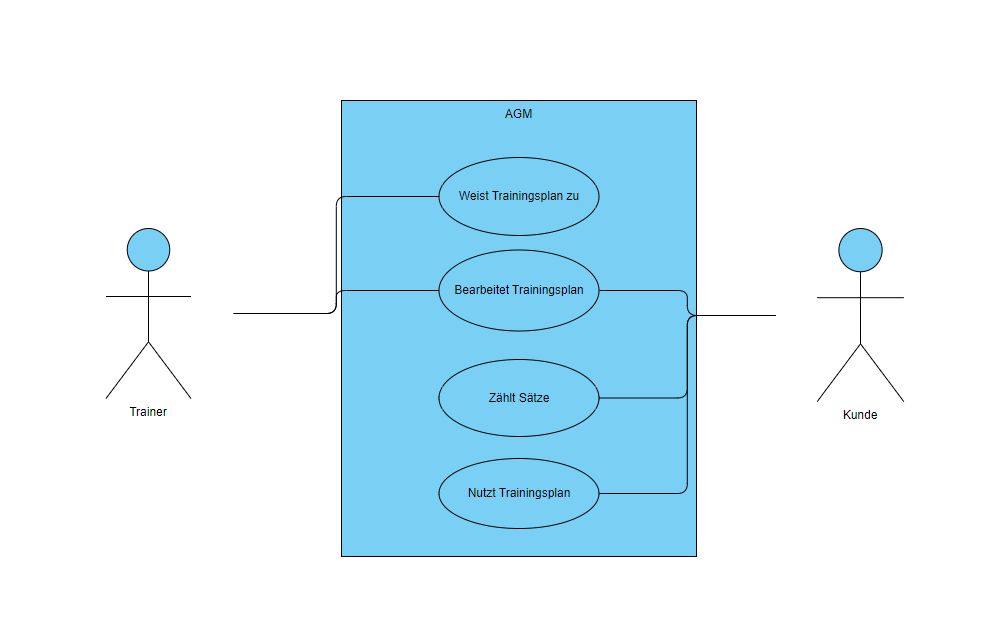
\includegraphics[scale=0.6]{pics/Use Case Diagramm.png}
        \caption{Use-Case Diagramm}
    \end{figure}


    \section{Entity Relationship Diagram - ERD}
    \setauthor{Antonio Kuvac}

    Ein ERD \cite{ERModell} ist ein Diagramm der Beziehungen (Relationship) zwischen Entitäten (Entity) in einem Datenbankschema darstellt. 
    Es wird verwendet, um das Design einer Datenbank zu modellieren und darzustellen und wie Daten in der Datenbank organisiert und miteinander verbunden sind.

    \pagebreak

    \subsection{Komponenten eines ERDs}

    Üblicherweise bestehen ERD-Diagramme aus drei Hauptkomponenten, und zwar aus Entitäten, Attributen und Beziehungen.

    \begin{itemize}
        \item Entitäten: Eine Entität repräsentiert eine Klasse von Objekten, die bestimmte Eigenschaften oder Attribute gemeinsam haben. Ein Beispiel für eine Entität wäre zum Beispiel ein Kunde der als Attribute einen Namen und eine Wohnadresse hat. Entitäten werden meistens als Rechtecke dargestellt
        \item Attribute: Attribute sind die Eigenschaften, die die Entitäten beschreiben, wie beispielsweise der Name eines Kunden oder die Menge eines Produkts. Attribute werden meistens durch Ellipsen dargestellt können aber auch in der Entität selbst drinnen stehen.
        \item Beziehungen: Beziehungen beschreiben die Art und Weise, wie Entitäten miteinander in Verbindung stehen. 
        Man unterscheidet zwischen drei Arten von Beziehungen. Die erste ist One-to-One.  Diese Beziehung tritt auf, wenn jeder Datensatz in der ersten Tabelle nur einen entsprechenden Datensatz in der zweiten Tabelle hat und umgekehrt. Ein Beispiel dazu wäre eine Person und sein Reisepass, denn jede Person hat nur einen Reisepass und ein Reisepass gehört nur zu einer Person.
        Die zweite Art ist One-to-Many. Diese Beziehung tritt auf, wenn ein Datensatz in der ersten Tabelle mehrere Datensätze in der zweiten Tabelle hat. Ein Beispiel dafür ist eine Mutter die mehrere Kinder hat, aber jedes Kind hat nur eine leibliche Mutter.
        Die Letzte Art von Beziehung ist Many-to-Many.Diese Beziehung tritt auf, wenn ein Datensatz in der ersten Tabelle mehrere Datensätze in der zweiten Tabelle hat, aber auch umgekehrt. Ein Beispiel für diese Beziehung ist ein Student der mehrere Kurse hat und ein Kurs der mehrere Studenten hat.

        \end{itemize}

        \pagebreak

    \subsection{Verwendung des Entity Relationship Diagrams in der Diplomarbeit}

    Um eine funktionierende Datenbank für das Backend zu gewährleisten wurde in Zusammenarbeit mit den Mitgliedern vom Projekt AberGym  mithilfe eines ERDs eine Datenbankstruktur erstellt die sowohl für die Anforderungen von AberGym als auch für die Anforderungen von AberGymMobile angepasst ist.

    \begin{figure}[H]
        \centering
        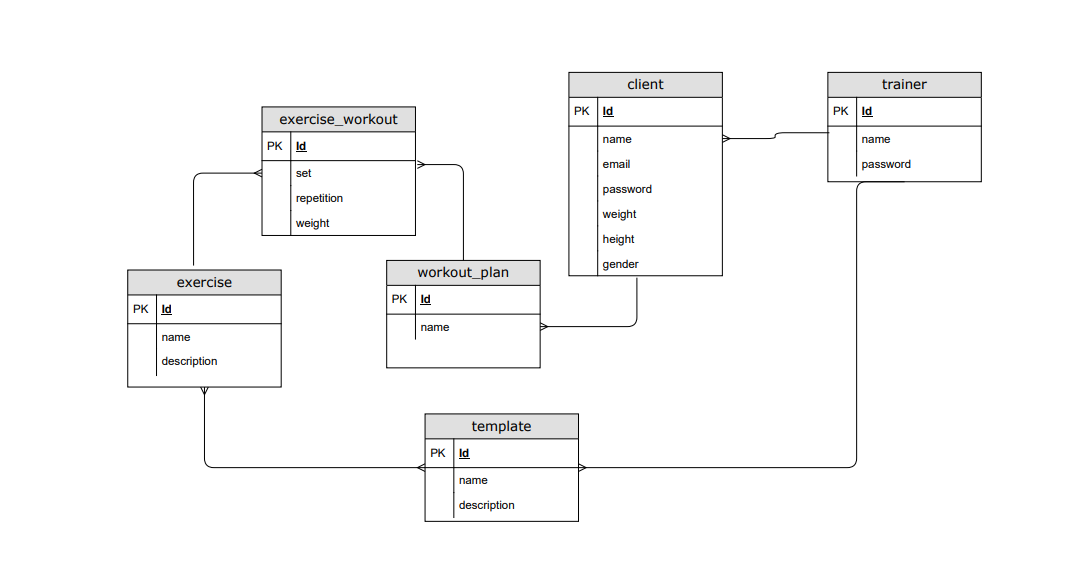
\includegraphics[scale=0.6]{pics/erd plantuml.png}
        \caption{ERD Diagramm in PlantUml}
    \end{figure}

    \subsection{PlantUml}
    PlantUML \cite{PlantUML} ist ein Open-Source-Tool zur Erstellung von UML-Diagrammen, das dabei unterstützt, Software-Architekturen, Systemdesigns und Prozessabläufe auf einfache Weise zu visualisieren. Es verwendet eine textbasierte Syntax, um Diagramme zu erstellen, die leicht verständlich, modifizierbar und in verschiedenen Formaten exportierbar sind. In diesem Text werden die wichtigsten Merkmale von PlantUML, seine Anwendungsbereiche sowie einige nützliche Ressourcen vorgestellt.

    \pagebreak
    \section{Design Thinking}
    \setauthor{Antonio Kuvac}


    Design Thinking \cite{DesignThinking} ist eine innovative Kreativitätstechnik, die in den letzten Jahren immer mehr an Bedeutung gewonnen hat. 
    Diese Methode verbindet kreative und analytische Ansätze, um komplexe Probleme zu lösen und innovative Lösungen zu entwickeln. 
    Design Thinking fördert dabei ein tiefes Verständnis für die Bedürfnisse der Nutzer*innen und stellt diese in den Mittelpunkt des Entwicklungsprozesses. 

   
    \subsection{Phasen des Design Thinking}

    Der Design-Thinking-Prozess besteht aus mehreren Phasen, die iterativ und flexibel durchlaufen werden. Diese Phasen sind:

    \begin{itemize}
        \item \textbf{Verstehen:} In dieser Phase geht es darum, das Problem, die Herausforderung oder den Kontext zu erfassen und ein tiefes Verständnis für die Bedürfnisse der Nutzer*innen zu entwickeln.
        \item \textbf{Beobachten:} Durch direkte Beobachtungen, Interviews und andere qualitative Methoden Informationen und Empathie für die Zielgruppe sammeln.
        \item \textbf{Sichten:} Die gesammelten Informationen werden analysiert, um Muster und Zusammenhänge zu erkennen. Hier werden auch Problemstellungen und Fragestellungen definiert.
        \item \textbf{Ideenfindung:} In dieser Phase werden verschiedene Kreativitätstechniken eingesetzt, um möglichst viele und vielfältige Ideen zu generieren.
        \item \textbf{Prototyping:} Die entwickelten Ideen werden in Form von einfachen und kostengünstigen Prototypen umgesetzt, um sie anschließend testen zu können.
        \item \textbf{Testen:} Die Prototypen werden mit der Zielgruppe getestet, um Feedback zu erhalten und die Lösungen kontinuierlich zu verbessern.
    \end{itemize}
    

    \subsection{Verwendung von Design Thinking in der Diplomarbeit}
    Design Thinking wurde während der Planungsphase und darüber hinaus kontinuierlich verwendet. 
    Durch häufige Meetings mit dem Betreuer und dem Projektpartner dieser Diplomarbeit haben Ideen und die Prototypen (Mockups) permanent Feedback erhalten und wurden dementsprechend angepasst und verbessert.

    \section{Brain Storming}
    \setauthor{Antonio Kuvac}

    Brainstorming \cite{Brainstorming} ist eine weit verbreitete und populäre Kreativitätstechnik, die darauf abzielt, eine Vielzahl von Ideen in kurzer Zeit zu generieren.

    \subsection{Prinzipien von Brainstorming}
    Das Brainstorming basiert auf einigen grundlegenden Prinzipien, die darauf abzielen, die kreative Zusammenarbeit zu fördern und die Entstehung neuer Ideen zu begünstigen. Zu diesen Prinzipien gehören:

    \begin{itemize}
        \item \textbf{Keine Kritik:} Während der Brainstorming-Sitzung sollte jegliche Kritik und Bewertung von Ideen vermieden werden.
        \item \textbf{Quantität geht vor Qualität:} In der Ideengenerierungsphase des Brainstormings ist das Hauptziel, möglichst viele Ideen zu sammeln, unabhängig von ihrer Qualität. Die Auswahl und Bewertung der Ideen erfolgt in einem späteren Schritt.
        \item \textbf{Kombination und Verbesserung von Ideen:} Man wird ermutigt auf bereits geäußerte Ideen aufzubauen und sie zu verbinden oder zu verbessern.
        \item \textbf{Freies Denken:} Brainstorming ist auf unkonventionelle und unerwartete Ideen ausgelegt um keine Ideen als unnötig einzustufen.
    \end{itemize}

    \subsection{Verwendung von Brainstorming in der Diplomarbeit}
    Nach jedem Meeting wurde Brainstorming angewandt um auf alle möglichen Ideen zu kommen. Wenn sich auf etwas geeinigt wurde, wurde es in die Tat umgesetzt, um Feedback dafür zu bekommen.

 \pagebreak

    \section{Kopfstand Methode}
    Die Kopfstand-Methode \cite{KopfstandMethode}, ist eine Kreativitätstechnik, die darauf abzielt, sich anstatt direkt auf die Lösung eines Problems zu konzentrieren,  Probleme aus einer negativen Perspektive zu betrachten.

    \begin{itemize}
        \item \textbf{Problemumkehr}: Das ursprüngliche Problem oder die Fragestellung wird in ihr Gegenteil umgeformt, um eine neue Perspektive zu gewinnen.
        
        \item \textbf{Ideengenerierung}: Es werden Ideen entwickelt, die auf die umgekehrte Problemstellung oder Fragestellung abzielen, und konzentrieren sich dabei auf die negativen Aspekte des Themas.
        
        \item \textbf{Umkehr der Lösungsansätze}: Die negativen Ideen werden zurück in positive Lösungsansätze umgewandelt.
        
        \item \textbf{Bewertung und Auswahl}: Die entwickelten Ideen und Lösungsansätze werden hinsichtlich ihrer Anwendbarkeit, Machbarkeit und Relevanz bewertet. Die vielversprechendsten Lösungen können dann weiter verfeinert und in die Praxis umgesetzt werden.
        \end{itemize}

        \subsection{Verwendung der Kopfstand Methode in der Diplomarbeit}
        Durch eine Kombination von anderen Kreativitätstechniken kamen immer Gedanken von Problemen wo sich die frage stellte , welche Probleme man mit gewissen Vorangehensweisen hätte. Somit wurde im Laufe der Planung mit der Kopfstand Methode abgewägt was in naher Zukunft an Problemen bereiten könnte und wie mit diesen Problemen umgegangen wird.  


\newpage
\section{Mockups}
\setauthor{Antonio Peric}  
Im Rahmen des Entwicklungsprozesses unserer mobilen Anwendung haben wir vier verschiedene Mockups erstellt, um das beste Design für die Nutzer*innen zu ermitteln und es optimal an die Bedürfnisse verschiedener Zielgruppen anzupassen. Die Gestaltung dieser Mockups berücksichtigt sowohl ästhetische als auch funktionale Aspekte, um eine ansprechende und effiziente Benutzeroberfläche zu schaffen, die den unterschiedlichen Anforderungen der*die Nutzer*innen gerecht wird.
\newline
\newline
Die vier Mockups wurden sorgfältig entworfen und auf Basis von Designprinzipien und Benutzeranforderungen entwickelt, um sicherzustellen, dass sie alle relevanten Funktionen und Interaktionen der Anwendung abbilden. Dabei wurde darauf geachtet, unterschiedliche Designansätze und Interaktionsmöglichkeiten zu berücksichtigen, um ein breites Spektrum an Nutzerpräferenzen abzudecken.
\newline
\newline
Nach einer umfassenden Analyse und Bewertung der vier Mockups haben unser Berater und Partner das vierte Mockup als das am besten geeignete Design ausgewählt. Dieses Design wurde aufgrund seiner benutzerfreundlichen Gestaltung, der klaren Struktur und der ansprechenden visuellen Elemente bevorzugt. Zudem wurde es als am ehesten in der Lage erachtet, die Bedürfnisse und Anforderungen der verschiedenen Zielgruppen zu erfüllen.

\newpage
Beim Öffnen der mobilen Anwendung gelangen die Nutzer*innen zunächst in den Log-in-Bereich (\hyperref[fig:log1]{siehe Abbildung 1}, \hyperref[fig:log2]{siehe Abbildung 2}). Hier besteht die Möglichkeit, sich mithilfe eines QR-Codes oder NFC-Technologie schnell und unkompliziert einzuloggen. Durch die Integration dieser modernen und benutzerfreundlichen Authentifizierungsmethoden wird der Zugang zur Anwendung für die Nutzer*innen erleichtert und die Sicherheit der persönlichen Daten gewährleistet.

\begin{figure}[!htb]
    \centering
    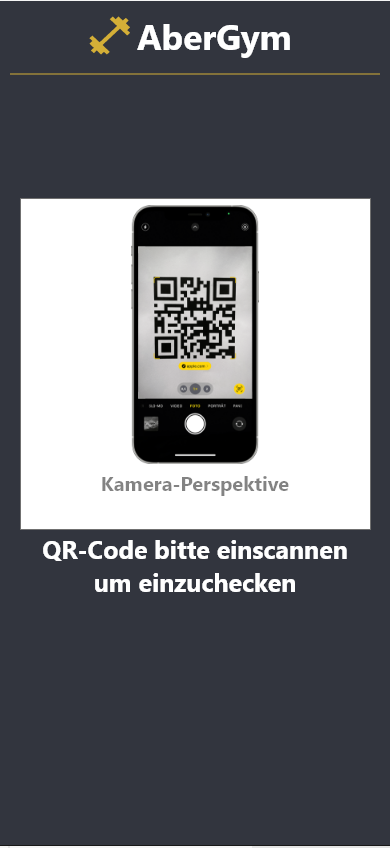
\includegraphics[width=0.35\textwidth]{pics/log1.png}
    \caption{Mockup 1 | Log-in-Bereich der mobilen Anwendung}
    \label{fig:log1}
\end{figure}
\begin{figure}[!htb]
    \centering
    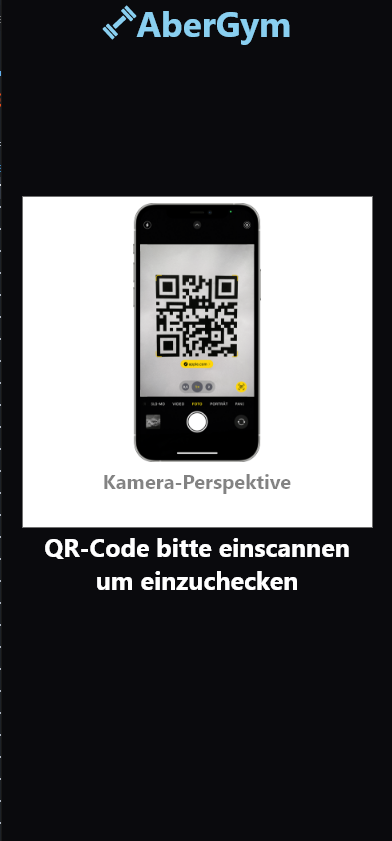
\includegraphics[width=0.35\textwidth]{pics/log2.png}
    \caption{Mockup 2 | Log-in-Bereich der mobilen Anwendung}
    \label{fig:log2}
\end{figure}
\FloatBarrier

Nach erfolgreichem Einloggen in die mobile Anwendung werden die Nutzer*innen automatisch zum heutigen Trainingsplan weitergeleitet. Dort besteht die Möglichkeit, den Trainingsplan jederzeit durch Berührung der Touchfläche {``Trainingsplan starten''} zu starten. Diese benutzerfreundliche Gestaltung ermöglicht einen schnellen Zugriff auf die wichtigsten Funktionen und erleichtert den Einstieg in das Training.
\newline
\newline
In der unteren Leiste, die in \hyperref[fig:main3]{Abbildung 3} und \hyperref[fig:main4]{siehe Abbildung 4} dargestellt ist, können die Nutzer*innen bequem zwischen dem letzten und dem heutigen Trainingsplan navigieren. Diese Funktion erleichtert den Zugriff auf vergangene und aktuelle Trainingspläne und bietet den Nutzer*innen eine flexible Möglichkeit, ihre Trainingshistorie und Fortschritte einzusehen und zu verwalten.

\begin{figure}[!htb]
    \centering
    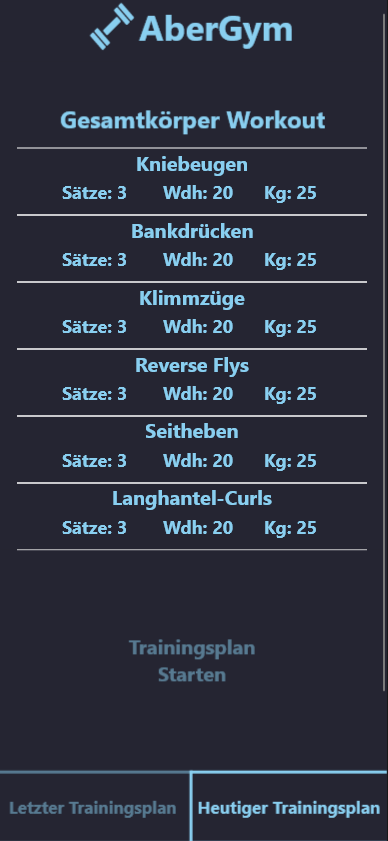
\includegraphics[width=0.35\textwidth]{pics/main3.png}
    \caption{Mockup 3 | Hauptbereich der mobilen Anwendung}
    \label{fig:main3}
\end{figure}
\begin{figure}[!htb]
    \centering
    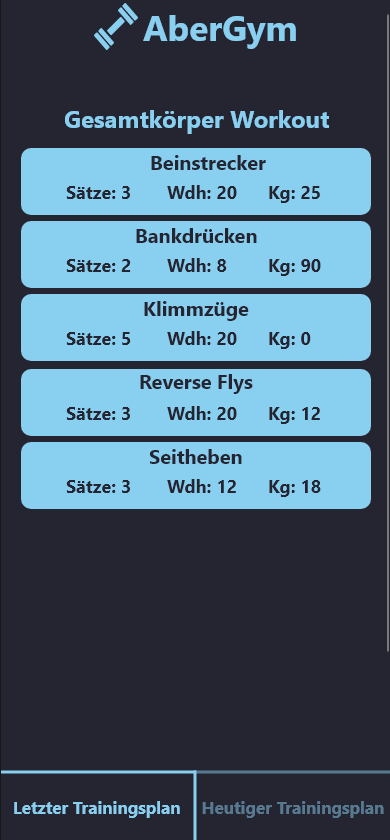
\includegraphics[width=0.35\textwidth]{pics/main4.png}
    \caption{Mockup 4 | Hauptbereich der mobilen Anwendung}
    \label{fig:main4}
\end{figure}
\FloatBarrier

Sobald die Nutzer*innen die Touchfläche {``Trainingsplan starten''} betätigen, wird der heutige Trainingsplan auf einer neuen Seite geöffnet und in einer To-Do-Ansicht präsentiert. In dieser Ansicht können die Nutzer*innen eine beliebige Übung auswählen und durchgehen. Zudem besteht die Möglichkeit, eine Übung zu bearbeiten, indem die Nutzer*innen die gewünschte Übung längere Zeit gedrückt halten. Diese flexible und benutzerfreundliche Gestaltung ermöglicht es den Nutzer*innen, ihren Trainingsplan individuell anzupassen und effizient durchzuarbeiten (\hyperref[fig:todolist1]{siehe Abbildung 5}, \hyperref[fig:todolist2]{siehe Abbildung 6}, \hyperref[fig:todolist3]{siehe Abbildung 7}, \hyperref[fig:todolist4]{siehe Abbildung 8}).

\begin{figure}[!htb]
    \centering
    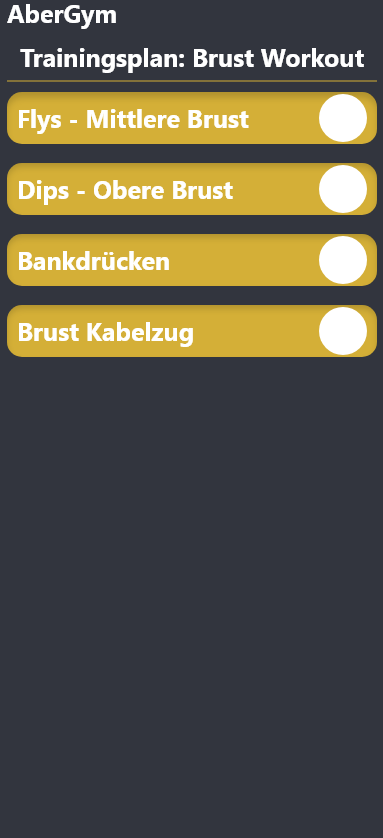
\includegraphics[width=0.35\textwidth]{pics/todolist1.png}
    \caption{Mockup 1 | To-Do-Bereich der mobilen Anwendung}
    \label{fig:todolist1}
\end{figure}
\begin{figure}[!htb]
    \centering
    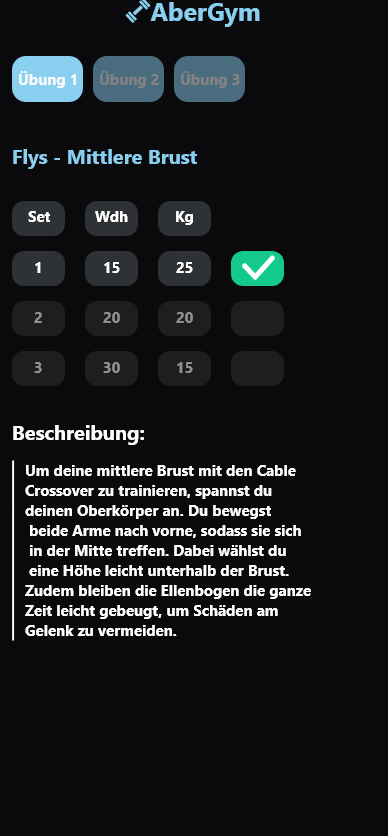
\includegraphics[width=0.35\textwidth]{pics/todolist2.png}
    \caption{Mockup 2 | To-Do-Bereich der mobilen Anwendung}
    \label{fig:todolist2}
\end{figure}
\begin{figure}[!htb]
    \centering
    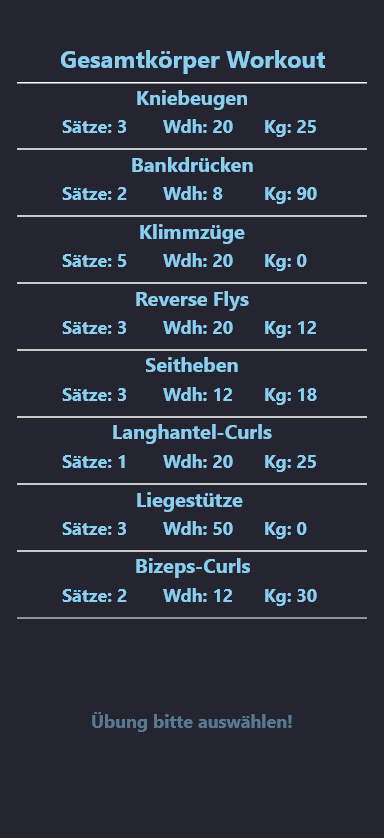
\includegraphics[width=0.35\textwidth]{pics/todolist3.png}
    \caption{Mockup 3 | To-Do-Bereich der mobilen Anwendung}
    \label{fig:todolist3}
\end{figure}
\begin{figure}[!htb]
    \centering
    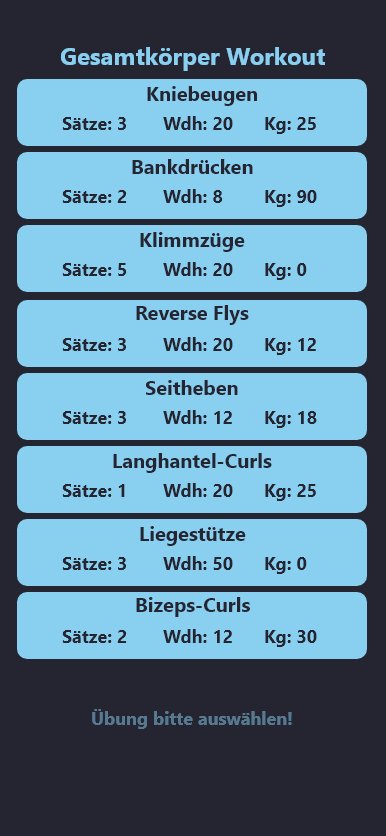
\includegraphics[width=0.35\textwidth]{pics/todolist4.png}
    \caption{Mockup 4 | To-Do-Bereich der mobilen Anwendung}
    \label{fig:todolist4}
\end{figure}
\FloatBarrier

Wenn die Nutzer*innen eine Übung auswählen, wird die entsprechende Übungsinformation erneut angezeigt. In jedem Mockup ist ein Zähler integriert, der bei Berührung des Bildschirms erhöht wird. Der gesamte Bildschirm dient als Druckfläche, um die Bedienung auch für Nutzer*innen mit Handschuhen zu erleichtern, da das Drücken von kleinen Buttons in solchen Situationen schwierig sein kann.
\newline
\newline
Sobald der Zähler den gleichen Wert wie die Satzanzahl der Übung erreicht hat, werden die Nutzer*innen automatisch zur To-Do-Ansicht zurückgeleitet. Die abgeschlossene Übung wird dann grau markiert und ans Ende der Liste verschoben. Dieses intuitive Design ermöglicht es den Nutzer*innen, ihren Fortschritt im Trainingsplan einfach nachzuvollziehen und sich auf die verbleibenden Übungen zu konzentrieren (\hyperref[fig:count1]{siehe Abbildung 9}, \hyperref[fig:todolist2]{siehe Abbildung 6}, \hyperref[fig:count3]{siehe Abbildung 11}, \hyperref[fig:count4]{siehe Abbildung 12}).

\begin{figure}[!htb]
    \centering
    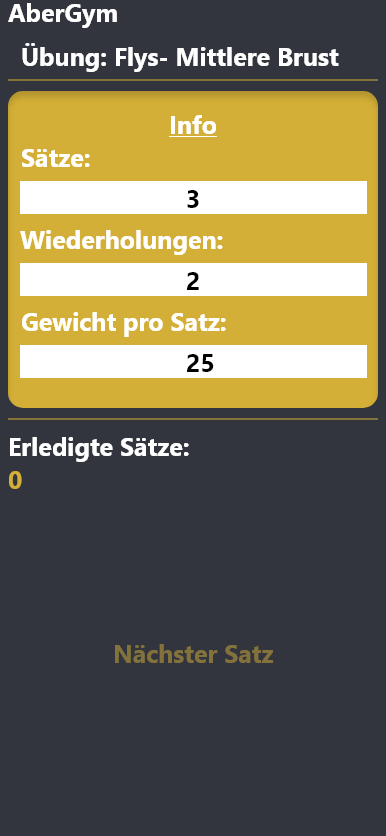
\includegraphics[width=0.35\textwidth]{pics/count1.png}
    \caption{Mockup 1 | Zähl-Bereich der mobilen Anwendung}
    \label{fig:count1}
\end{figure}
\begin{figure}[!htb]
    \centering
    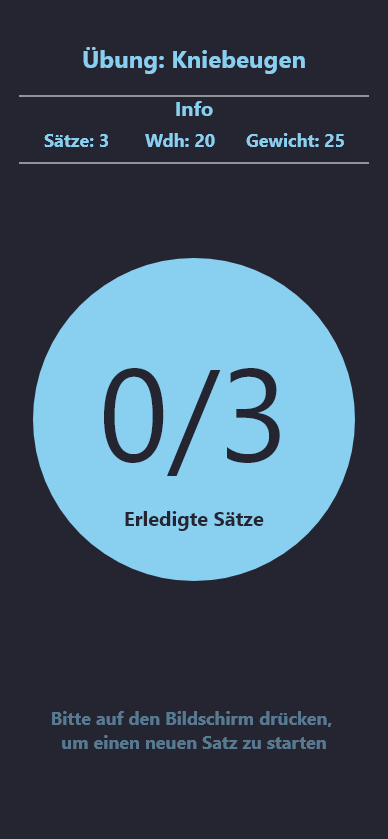
\includegraphics[width=0.35\textwidth]{pics/count3.png}
    \caption{Mockup 3 | Zähl-Bereich der mobilen Anwendung}
    \label{fig:count3}
\end{figure}
\begin{figure}[!htb]
    \centering
    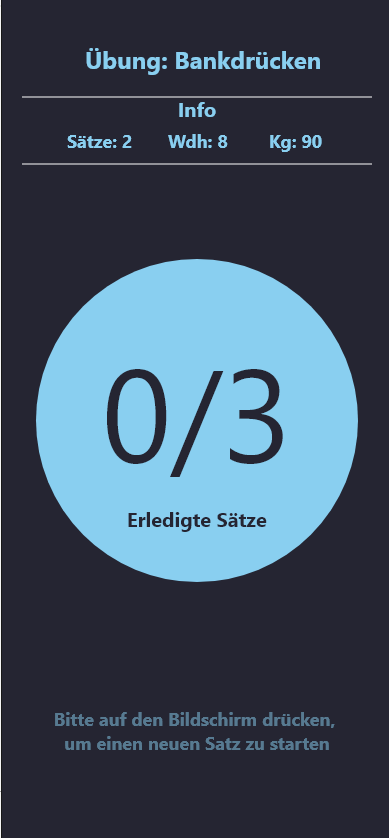
\includegraphics[width=0.35\textwidth]{pics/count4.png}
    \caption{Mockup 4 | Zähl-Bereich der mobilen Anwendung}
    \label{fig:count4}
\end{figure}
\FloatBarrier

Sobald die Nutzer*innen alle Übungen abgeschlossen haben, werden sie zur Hauptseite zurückgeleitet, auf der sie die vorgenommenen Änderungen während der Durchführung des Trainingsplans einsehen können. Der aktualisierte Trainingsplan, der die neuen Werte der jeweils bearbeiteten Übungen enthält, wird unter der Navigation "Heutiger Trainingsplan" angezeigt. Die Nutze*rinnen können den überarbeiteten Trainingsplan erneut durcharbeiten, indem sie die Touchfläche {``Trainingsplan starten''} betätigen.
\newline
\newline
In der Navigation "Letzter Trainingsplan" wird hingegen der ursprüngliche Trainingsplan mit den alten Daten der jeweiligen bearbeiteten Übungen dargestellt. Dieser kann jedoch nicht erneut gestartet werden. Diese Funktion ermöglicht den Nutzer*innen, die Fortschritte und Veränderungen im Trainingsplan nachzuvollziehen und die Entwicklung ihrer Trainingsergebnisse im Zeitverlauf zu verfolgen (\hyperref[fig:finished3]{siehe Abbildung 13}, \hyperref[fig:finished4]{siehe Abbildung 14}).

\begin{figure}[!htb]
    \centering
    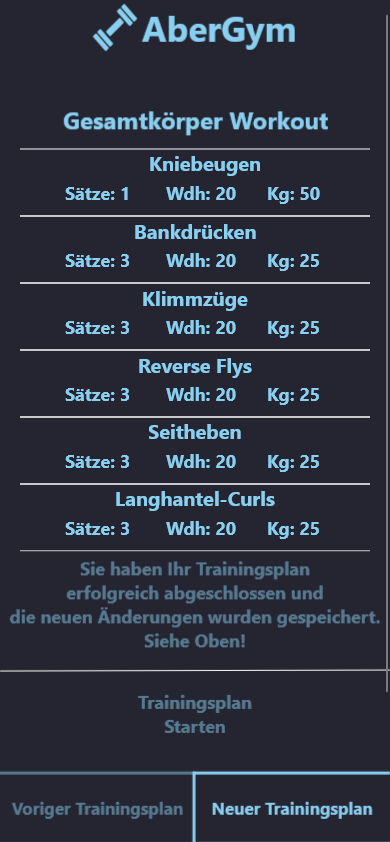
\includegraphics[width=0.35\textwidth]{pics/finished3.png}
    \caption{Mockup 3 | Hauptbereich nach der Durcharbeitung des Trainingplans}
    \label{fig:finished3}
\end{figure}
\begin{figure}[!htb]
    \centering
    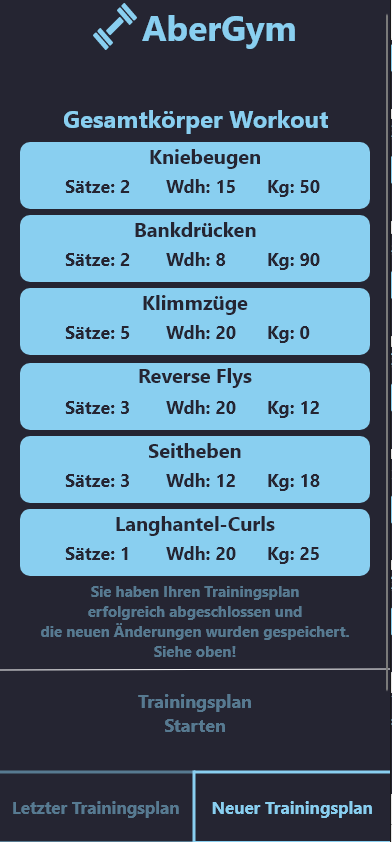
\includegraphics[width=0.35\textwidth]{pics/finished4.png}
    \caption{Mockup 4 | Hauptbereich nach der Durcharbeitung des Trainingplans}
    \label{fig:finished4}
\end{figure}
\FloatBarrier

Obwohl das Mockup 4 ursprünglich ausgewählt wurde, wurde während des Entwicklungsprozesses das Design weiter angepasst, optimiert und verschönert. Diese Änderungen wurden vorgenommen, um den Nutzer*innen die Navigation innerhalb der App zu erleichtern und ihnen dabei zu helfen, sich besser zurechtzufinden. Durch diese Designanpassungen wurde eine benutzerfreundliche und ansprechende Oberfläche geschaffen, die den Bedürfnissen und Erwartungen der-die Nutzer-innen entspricht.	

\begin{spacing}{1}
\chapter{Technologien}\label{chapter:tech}
\end{spacing}
\section{Flutter}
\setauthor{Antonio Peric}

Flutter ist ein Open-Source UI-Toolkit von Google zur Entwicklung von Anwendungen für mobile Geräte, Desktop-Computer und das Web. Es basiert auf der Programmiersprache Dart und verwendet eine Vielzahl von Widgets und Tools, um eine schnelle Entwicklung und hohe Qualität zu ermöglichen. Flutter ermöglicht es Entwicklern, attraktive und benutzerfreundliche Anwendungen zu erstellen, die auf verschiedenen Plattformen laufen können 
\cite{aws-flutter}.
\subsection{Entwicklungs-Ergonomie}

Flutter bietet eine sehr gute Entwicklungs-Ergonomie durch eine intuitive Benutzeroberfläche und eine umfassende Dokumentation. Die Widgets und Tools von Flutter sind gut strukturiert und können einfach angepasst werden. Darüber hinaus ermöglicht Flutter eine schnelle Erstellung von Prototypen und eine schnelle Iteration, was die Entwicklung von Anwendungen beschleunigt.

\subsection{Tiefgehende Codeanalyse}

Flutter bietet tiefgehende Codeanalysefunktionen, die Entwicklern helfen, Fehler schnell zu finden und zu beheben. Die Analysefunktionen umfassen eine statische Analyse, die Probleme wie Typfehler, fehlende Importe und andere Fehler aufdeckt, bevor die Anwendung ausgeführt wird. Flutter bietet auch eine dynamische Analyse, die Probleme während der Laufzeit aufdeckt.
\newpage

\subsection{Effiziente Navigation und Suche}

Flutter bietet eine effiziente Navigation und Suche, die es Entwicklern ermöglicht, schnell durch den Code zu navigieren und Probleme zu finden. Die IDEs, die Flutter unterstützen, wie beispielsweise IntelliJ IDEA, Visual Studio Code und Android Studio, bieten eine schnelle Navigation durch den Code sowie eine leistungsstarke Suche nach Dateien und Zeilen.

\subsection{Entwicklung: Ausführen, Testen, Debuggen}

Flutter ermöglicht Entwicklern eine effiziente Entwicklung, indem es ein integriertes Debugging- und Test-Framework bietet. Entwickler können ihre Anwendungen in Echtzeit testen und debuggen, ohne die Anwendung manuell neu starten zu müssen. Das Testen von Anwendungen ist ebenfalls einfach und kann durch den Einsatz von Frameworks wie Flutter Test und Mockito unterstützt werden.

\subsection{Funktionen}

Flutter bietet zahlreiche Funktionen und Tools, um Entwicklern bei der Entwicklung von Anwendungen zu helfen. Hier sind einige der wichtigsten Funktionen:

\begin{itemize}
\item Widgets: Flutter bietet eine große Auswahl an vorgefertigten Widgets, die Entwickler verwenden können, um benutzerdefinierte Benutzeroberflächen zu erstellen.
\item Hot Reload: Mit Hot Reload können Entwickler Änderungen an der Anwendung vornehmen und diese Änderungen sofort überprüfen, ohne die Anwendung neu starten zu müssen.
\item State Management: Flutter bietet eine Vielzahl von State-Management-Lösungen, einschließlich Provider und Redux, die es Entwicklern ermöglichen, den Zustand ihrer Anwendung effizient zu verwalten.
\item Plattformunabhängigkeit: Flutter ist plattformunabhängig und ermöglicht es Entwicklern, eine Anwendung zu erstellen, die auf verschiedenen Plattformen ausgeführt werden kann, einschließlich Android, iOS, Web und Desktop.
\newpage
\item Performance: Flutter ist schnell und leistungsfähig und bietet eine schnelle Animation und flüssige Benutzeroberflächen, ohne Einbußen bei der Performance. Durch die Verwendung von Skia, einer 2D-Grafik-Engine, können Entwickler hochwertige Animationen und visuell ansprechende Benutzeroberflächen erstellen, die auf verschiedenen Geräten einheitlich und flüssig funktionieren.
\end{itemize}

\subsection{Vorteile}
Flutter bietet mehrere Vorteile:

\begin{compactitem}
    \item \textbf{Plattformübergreifende Entwicklung}: Mit Flutter können Entwickler plattformübergreifende Anwendungen erstellen, die auf verschiedenen Betriebssystemen wie iOS, 
    Android, Web und Desktop laufen. Dies reduziert die Entwicklungskosten und spart Zeit und Ressourcen.
    \item \textbf{Schnelle Entwicklung}: Flutter bietet die Funktion "Hot Reload", die es Entwickler*innen ermöglicht, Änderungen in Echtzeit zu sehen, 
    ohne die Anwendung neu starten zu müssen. Dadurch wird die Entwicklung von Flutter-Anwendungen schneller und effizienter.
    \item \textbf{Reaktionsfähigkeit}: Flutter-Anwendungen sind schnell und reaktionsfähig, da sie auf der leistungsstarken Grafik-Engine Skia basieren. 
    Dies ermöglicht es Entwickler*innen, reibungslose Benutzererfahrungen mit flüssigen Animationen und Grafiken zu schaffen.
    \item \textbf{Einfache UI-Erstellung}: Mit der eigenen Widget-Bibliothek von Flutter können Entwickler*innen schnell und einfach ansprechende Benutzeroberflächen erstellen. 
    Die Bibliothek enthält viele vorgefertigte Widgets, die einfach angepasst werden können.
    \item \textbf{Native Performance}: Flutter-Anwendungen werden in nativem Code ausgeführt, was zu einer höheren Leistung und Geschwindigkeit führt als bei Hybrid- oder webbasierten Anwendungen.
\end{compactitem}

\newpage
\section{Dart als Programmiersprache}
Dart ist eine objektorientierte Programmiersprache, die von Google entwickelt wurde und erstmals im Jahr 2011 vorgestellt wurde. Im Vergleich zu anderen Sprachen wie Java, Python und C++ ist Dart eine vergleichsweise neue Programmiersprache. Sie wurde entwickelt, um die Herausforderungen bei der Entwicklung von Webanwendungen zu bewältigen und ist auch für die Entwicklung von plattformübergreifenden mobilen Anwendungen geeignet \cite{aws-flutter}.

\subsection{Statische Typisierung}
Eine der wichtigsten Eigenschaften von Dart ist die statische Typisierung. Statische Typisierung bedeutet, dass Variablen und Funktionen vor der Laufzeit überprüft werden. Dadurch können Entwickler*innen Fehler frühzeitig erkennen und vermeiden. Statische Typisierung verbessert auch die Lesbarkeit und Wartbarkeit des Codes.

\subsection{Dynamische Typisierung}
Dart unterstützt auch dynamische Typisierung. Diese Funktion erleichtert die Entwicklung von Anwendungen, die auf sich ändernden Datenstrukturen basieren. Mit der dynamischen Typisierung kann der Code flexibler gestaltet werden und Entwickler*innen können schneller auf Änderungen reagieren.

\subsection{Funktionale Programmierung}
Dart unterstützt auch funktionale Programmierung, die eine saubere und lesbare Codebasis fördert. Die Verwendung von Funktionen als Parameter erhöht die Flexibilität und Wiederverwendbarkeit von Code.

\subsection{Asynchrone Programmierung}
Dart unterstützt asynchrone Programmierung, um die Leistung bei der Verarbeitung von Netzwerk- und E/A-Operationen zu verbessern. Mit der asynchronen Programmierung können Entwickler*innen Anwendungen entwickeln, die schnell und effizient arbeiten und auf die Bedürfnisse der*die Benutzer*innen reagieren.

\subsection{Widgets}

Ein zentraler Bestandteil von Flutter sind Widgets. Widgets sind die Bausteine für die Erstellung von Benutzeroberflächen in Flutter. Sie sind leichtgewichtig und anpassbar und ermöglichen es Entwicklern, komplexe Benutzeroberflächen mit wenig Code zu erstellen. Es gibt eine große Auswahl an vorgefertigten Widgets in Flutter, die Entwickler verwenden können, um schnell und einfach eine benutzerdefinierte Benutzeroberfläche zu erstellen.

Flutter bietet auch die Möglichkeit, eigene Widgets zu erstellen. Dies gibt Entwicklern mehr Flexibilität und Kontrolle über die Benutzeroberfläche ihrer Anwendung. Darüber hinaus können Widgets in Flutter einfach angepasst werden, um sie an die Anforderungen der Anwendung anzupassen.

\subsection{State Management}

Die Verwaltung des Zustands ist ein wichtiger Aspekt bei der Entwicklung von Anwendungen. In Flutter gibt es verschiedene Möglichkeiten, den Zustand einer Anwendung effizient zu verwalten. Die am häufigsten verwendeten Lösungen für das State Management in Flutter sind Provider und Redux.

Provider ist eine einfachere Lösung für das State Management, die es Entwicklern ermöglicht, den Zustand ihrer Anwendung zu verwalten, ohne zusätzliche Bibliotheken hinzufügen zu müssen. Es ist eine leichtgewichtige Lösung, die die Verwaltung des Zustands vereinfacht und die Leistung der Anwendung verbessert.

Redux ist eine robuste Lösung für das State Management in Flutter, die Entwicklern eine hohe Kontrolle über den Zustand ihrer Anwendung bietet. Redux ist eine Bibliothek, die es Entwicklern ermöglicht, den Zustand ihrer Anwendung zentralisiert zu verwalten. Es bietet auch eine Vielzahl von Werkzeugen und Funktionen, um die Verwaltung des Zustands zu erleichtern.
\newpage
\subsection{Vorteile von Dart}

Dart bietet eine Reihe von Vorteilen für Entwickler, darunter:

\begin{itemize}
\item \textbf{Effiziente Ausführung}: Dart ist eine schnelle und leistungsfähige Sprache, die eine effiziente Ausführung von Anwendungen ermöglicht.
\item \textbf{Statische Typisierung}: Dart ist eine statisch typisierte Sprache, die Entwicklern hilft, Fehler frühzeitig zu erkennen und zu beheben.
\item \textbf{Flexibilität}: Dart unterstützt dynamische Typisierung, was Entwicklern Flexibilität bei der Entwicklung von Anwendungen bietet, die auf sich ändernden Datenstrukturen basieren.
\item \textbf{Asynchrone Programmierung}: Dart unterstützt asynchrone Programmierung, um die Leistung bei der Verarbeitung von Netzwerk- und E/A-Operationen zu verbessern.
\item \textbf{Wiederverwendbarkeit von Code}: Dart bietet die Möglichkeit, Funktionen als Parameter zu übergeben, um die Wiederverwendbarkeit von Code zu erhöhen.
\item \textbf{Einfach zu erlernen}: Dart ist eine relativ einfache Sprache, die schnell erlernt werden kann.
\item \textbf{Integration mit Flutter}: Dart wird von Flutter unterstützt und bietet Entwicklern eine leistungsstarke und effiziente Möglichkeit, plattformübergreifende Anwendungen zu entwickeln.
\end{itemize}

\pagebreak
\section{Visual Studio Code}
\setauthor{Antonio Kuvac}
Visual Studio Code ist ein kostenloses, plattformübergreifendes Code-Editor-Tool von Microsoft. Es ist ein beliebtes Tool für Entwickler*innen, 
da es eine Vielzahl von Funktionen und Erweiterungen bietet, um die Produktivität und Effizienz zu verbessern.

Visual Studio Code bietet eine intuitive Benutzeroberfläche, die es Entwickler*innen erleichtert, schnell und einfach zu navigieren und Code zu schreiben. 
Es bietet auch integrierte Debugging-Tools, die Entwickler*innen helfen, Fehler zu finden und zu beheben, sowie integrierte Versionskontrolltools für Git, 
um Änderungen am Code effektiv zu verwalten.

\subsection{Extensions}
Eine der wesentlichsten Funktionen in VS Code sind Extensions (Erweiterungen). VS Code-Extensions können verschiedene Funktionen bieten, 
wie z.B. Syntax-Hervorhebung, Autovervollständigung, Debugging-Tools, Git-Integration und vieles mehr. 
Es gibt eine breite Palette von Erweiterungen, die für verschiedene Programmiersprachen und Frameworks verfügbar sind, 
um die Entwicklungserfahrung zu verbessern und die Produktivität zu steigern.

Die Installation von VS Code-Extensions ist einfach und unkompliziert. Sie können über den Visual Studio Code-Marktplatz oder direkt aus der Editor-Benutzeroberfläche installiert werden.
Nach der Installation stehen die neuen Funktionen und Tools sofort zur Verfügung.
\pagebreak
\section{Docker}
\setauthor{Antonio Kuvac}
Docker ist eine Open-Source-Plattform, die es Entwicklern ermöglicht, Anwendungen in isolierten Containern zu erstellen, bereitzustellen und auszuführen. 
Docker-Container sind leichtgewichtig und portabel und bieten eine effektive Möglichkeit, Anwendungen in verschiedenen Umgebungen und Infrastrukturen auszuführen.

\subsection{Funktionsweise}
Docker verwendet Container, um Anwendungen zu isolieren und eine konsistente Umgebung für ihre Ausführung zu schaffen. Container sind ähnlich wie virtuelle Maschinen, 
jedoch leichter und schneller zu erstellen, da sie den Kernel des Host-Betriebssystems nutzen. Jeder Container enthält alles, was eine Anwendung zum Ausführen benötigt, 
einschließlich des Codes, der Abhängigkeiten und der Konfiguration.

Die Funktionsweise von Docker basiert auf einem Schichtmodell, das aus drei Komponenten besteht:

\begin{enumerate}
    \item \textbf{Docker Engine}: Dies ist das Kernstück von Docker und besteht aus dem Docker-Daemon und der Docker-CLI (Command Line Interface). Der Docker-Daemon ist ein Hintergrundprozess, 
    der die Verwaltung und Ausführung von Containern übernimmt, während die Docker-CLI als Schnittstelle für den Benutzer dient, um mit dem Docker-Daemon zu interagieren.
    \item \textbf{Images}: Ein Docker-Image ist eine Vorlage oder Blaupause für die Erstellung von Containern. 
    Es enthält den Code, die Abhängigkeiten und Konfigurationen einer Anwendung sowie alle anderen erforderlichen Komponenten, die zur Ausführung der Anwendung benötigt werden. 
    Docker-Images werden über Docker Files erstellt, die eine Liste von Anweisungen enthalten, um das Image zu konfigurieren und zu erstellen.
    \item \textbf{Container}: Ein Docker-Container ist eine Instanz eines Docker-Images, die ausgeführt wird. Ein Container kann gestartet, gestoppt und gelöscht werden. 
    Jeder Container ist isoliert und hat seine eigene Dateisystemumgebung, Netzwerkschnittstellen und Ressourcenlimits.
    \end{enumerate}

    \begin{figure}[H]
        \centering
        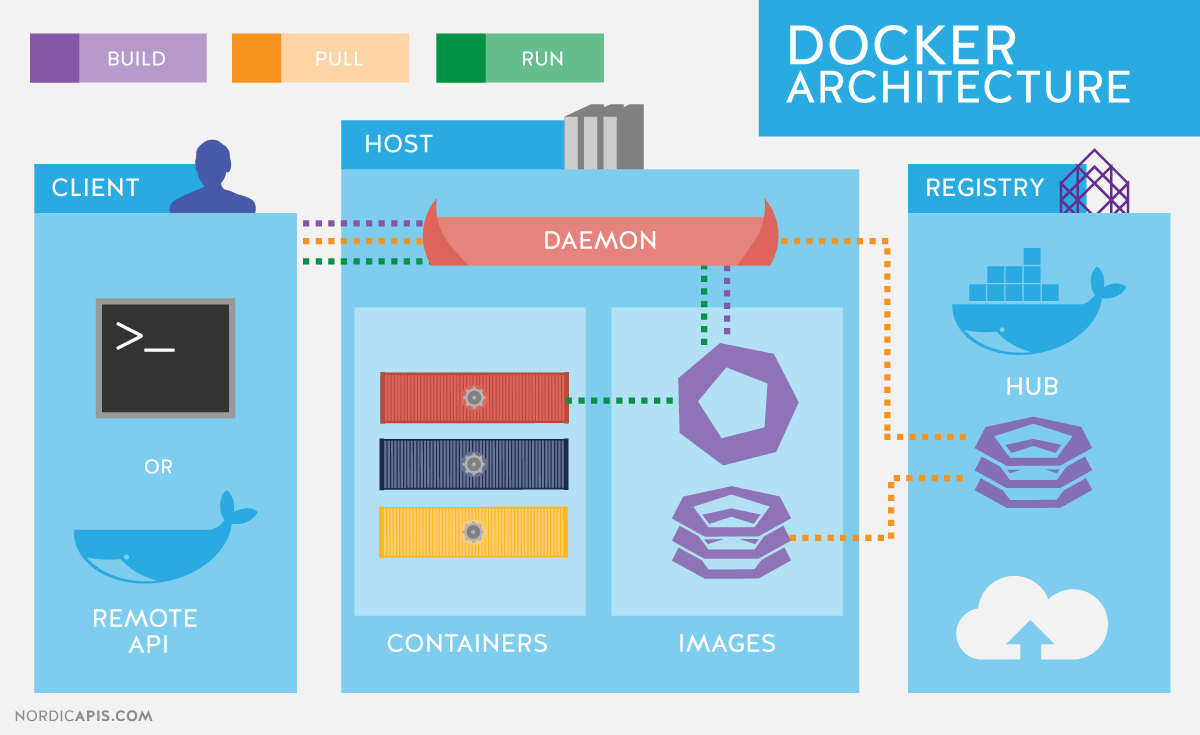
\includegraphics[scale=0.3]{pics/Docker_Architecture.png}
        \caption{Docker Architektur}
    \end{figure}

\subsection{Vorteile}
\begin{itemize}
    \item \textbf{Portabilität}: Docker-Container sind plattformunabhängig und können auf verschiedenen Betriebssystemen und Infrastrukturen ausgeführt werden.
    
    \item \textbf{Flexibilität}: Mit Docker können Anwendungen schnell erstellt, abgeändert und bereitgestellt werden, ohne die zugrunde liegende Infrastruktur ändern zu müssen.
    
    \item \textbf{Skalierbarkeit}: Docker ermöglicht eine einfache horizontale Skalierung von Anwendungen, indem es das Erstellen und Bereitstellen von Containern automatisiert.
    
    \item \textbf{Sicherheit}: Docker bietet Sicherheitsfunktionen wie Isolation und eingeschränkte Ressourcenkontrolle, um eine sicherere Ausführung von Anwendungen zu gewährleisten.
    
    \item \textbf{Effizienz}: Docker-Container sind leicht und benötigen weniger Ressourcen als virtuelle Maschinen, was zu einer höheren Effizienz und Leistung führt.
    \end{itemize}

    \section{Android Studio}
    \setauthor{Antonio Kuvac}
    Android Studio ist eine integrierte Entwicklungsumgebung (IDE), die speziell für die Entwicklung von Android-Apps entwickelt wurde. 
    Es wurde von Google entwickelt und ist kostenlos für Entwickler verfügbar, um Android-Apps zu erstellen und zu bearbeiten.

    \subsection{Funktionen}
    Android Studio verfügt über eine Vielzahl von Funktionen, die dabei helfen, schneller und effizienter Android-Apps zu entwickeln. Zu den wichtigsten Funktionen gehören:

    \begin{itemize}
        \item \textbf{Intelligentes Code-Editing:} Android Studio bietet intelligentes Code-Editing mit automatischen Vorschlägen, Fehlererkennung und Refactoring-Funktionen.
        \item \textbf{Emulator:} Entwickler können den Android-Emulator nutzen, um ihre Apps auf verschiedenen Android-Geräten zu testen, ohne physische Geräte besitzen zu müssen.
        \item \textbf{Layout-Editor:} Android Studio verfügt über einen Layout-Editor, mit dem Entwickler die Benutzeroberfläche ihrer Apps visuell gestalten können.
        \item \textbf{Gradle Build-System:} Android Studio verwendet das Gradle Build-System, das Entwicklern ermöglicht, komplexe Abhängigkeiten und Builds zu verwalten.
        \item \textbf{Integration mit anderen Tools:} Android Studio ist nahtlos in andere Google-Tools wie Firebase und Google Cloud Platform integriert.
        \end{itemize}

    \subsection{Emulator}
    Der Android Studio Emulator ist ein wichtiges Tool für Android-Entwickler, das es ihnen ermöglicht, ihre Apps auf verschiedenen Android-Geräten zu testen, ohne physische Geräte besitzen zu müssen. Der Emulator wird mit Android Studio mitgeliefert und kann einfach über die IDE gestartet werden.

Einer der größten Vorteile des Emulators ist, dass Entwickler ihre Apps auf verschiedenen Android-Versionen und Gerätekonfigurationen testen können, um sicherzustellen, 
dass ihre Apps auf allen unterstützten Geräten reibungslos funktionieren. 
Der Emulator kann eine Vielzahl von Android-Versionen und -Gerätekonfigurationen emulieren, einschließlich verschiedener Bildschirmauflösungen und -größen, 
Prozessortypen und Speicherkapazitäten.

Ein weiterer Vorteil des Emulators ist, dass er den Entwicklungsprozess beschleunigen kann, indem er den Build- und Bereitstellungsprozess verkürzt. 
Anstatt jedes Mal eine neue Version der App auf einem physischen Gerät zu testen, können Entwickler die App einfach im Emulator starten und testen, 
was Zeit spart und die Entwicklungszeit verkürzt.

Die Einrichtung des Emulators in Android Studio ist einfach und erfordert nur wenige Schritte. Entwickler müssen zunächst sicherstellen, 
dass sie die neueste Version von Android Studio heruntergeladen und installiert haben. Sobald sie Android Studio geöffnet haben, können sie den Emulator über das AVD Manager-Tool starten, 
das im Menü "Werkzeuge" zu finden ist.

Es gibt jedoch auch einige Nachteile beim Verwenden des Emulators. Einer der größten Nachteile ist die Geschwindigkeit. Da der Emulator ein virtuelles Gerät ist, 
kann er langsamer sein als ein physisches Gerät. Dies kann dazu führen, dass Entwickler länger warten müssen, um ihre Apps im Emulator zu testen.

Ein weiterer Nachteil ist, dass der Emulator nicht alle Funktionen eines physischen Geräts emulieren kann. Beispielsweise kann der Emulator keine Anrufe oder Textnachrichten empfangen und senden, 
da er kein physisches Mobilfunkmodem hat. Dies bedeutet, dass Entwickler nicht alle Aspekte ihrer App im Emulator testen können und gegebenenfalls auf physische Geräte zurückgreifen müssen.

Zusammenfassend lässt sich sagen, dass der Android Studio Emulator ein wertvolles Tool für Android-Entwickler ist, um ihre Apps auf verschiedenen Geräten und Android-Versionen zu testen. 
Obwohl der Emulator einige Nachteile hat, überwiegen die Vorteile in den meisten Fällen und er ist ein unverzichtbares Werkzeug für die App-Entwicklung.

\begin{figure}[H]
    \centering
    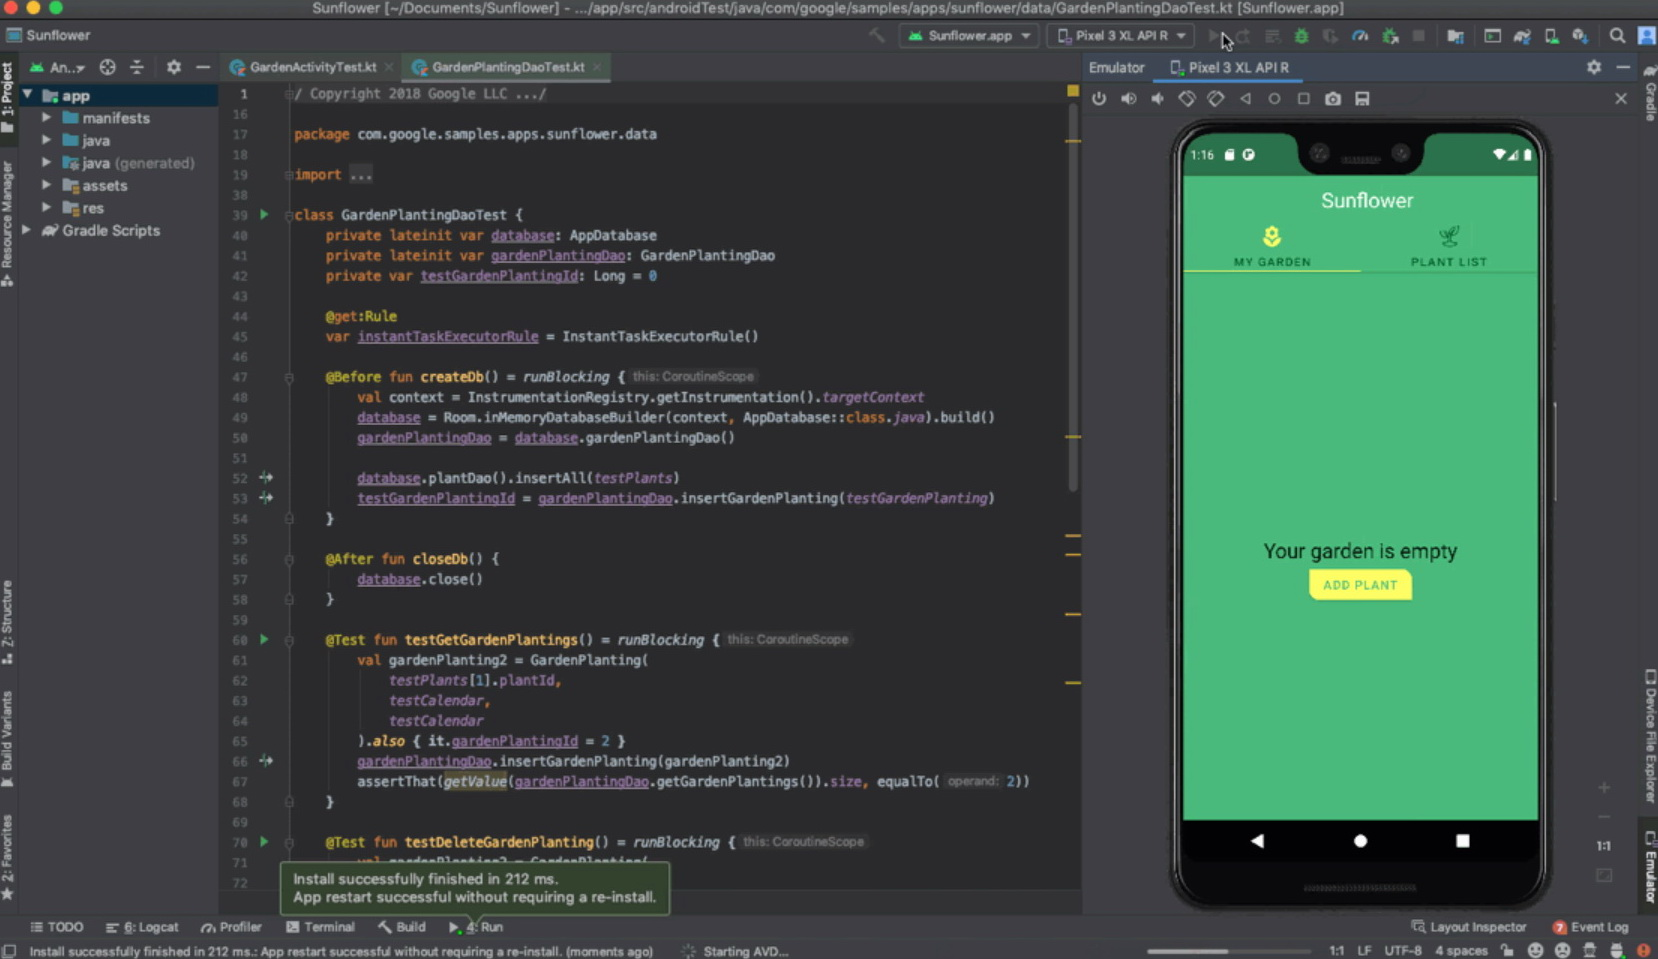
\includegraphics[scale=0.2]{pics/android-studio-emulator.jpg}
    \caption{Android Studio Emulator}
\end{figure}

\section{AdobeXD}
    \setauthor{Antonio Kuvac}

    AdobeXD ist eine Design-Software, die speziell für die Erstellung von Benutzeroberflächen und Interaktionen für Mobile Apps, Webseiten und andere digitale Plattformen entwickelt wurde.

\subsection*{Funktionen}
Die wichtigsten Funktionen sind intuitive Layout-Tools, um Entwürfe schnell zu erstellen und zu bearbeiten, Vektor-Tools, um hochwertige Grafiken zu erstellen, Prototyping-Funktionen, um interaktive Prototypen zu erstellen und zu testen und die Möglichkeit, Designs in Echtzeit zu teilen und Feedback von Stakeholdern zu erhalten.

\subsection*{Plattformübergreifendes Design} 
AdobeXD unterstützt plattformübergreifendes Design, was bedeutet, dass man nur eine einzige Design-Datei erstellen muss, um diese dann auf AdobeXD auf verschiedenen Geräten und Plattformen verwenden zu können. 
Das ermöglicht, schnell und effizient Designs für verschiedene Geräte und Plattformen zu erstellen.

\subsection*{Integration mit anderen Tools} 
AdobeXD ist nahtlos in andere Adobe-Tools wie Photoshop und Illustrator integriert. Das ermöglicht, Designs nahtlos zwischen verschiedenen Adobe-Tools zu übertragen. 
Es ist auch in andere Tools wie Slack und Microsoft Teams integriert, um die Zusammenarbeit zu erleichtern.

\subsection*{Cloud-basierte Zusammenarbeit} 
AdobeXD bietet eine Cloud-basierte Zusammenarbeit an, mit der es möglich ist, Designs in Echtzeit zu teilen und Feedback von Stakeholdern zu erhalten. 
Designer*innen können Links zu ihren Designs freigeben und Stakeholder können Kommentare und Feedback direkt in die Designs geben.

\section{IntelliJ IDEA}
\setauthor{Antonio Peric}

\textbf{IntelliJ IDEA} ist eine leistungsstarke und vielseitige Entwicklungsumgebung, die von Entwicklern auf der ganzen Welt genutzt wird. Mit der Fähigkeit, eine Vielzahl von Programmiersprachen zu unterstützen, hat es sich zu einem wichtigen Werkzeug für die Softwareentwicklung entwickelt.

Die Free-Version von IntelliJ IDEA bietet Unterstützung für Programmiersprachen wie Java, Groovy, Kotlin und Scala sowie Standardsyntaxsprachen wie XML. Mit dieser Version können Entwickler grundlegende Projekte erstellen und debuggen. Die Ultimate-Version von IntelliJ IDEA bietet jedoch erweiterte Funktionen, wie beispielsweise die Integration mit Frameworks, eine größere Auswahl an Plugins, Code-Refactoring-Tools und viele weitere Funktionen, die die Produktivität von Entwicklern erhöhen.

Für Schüler*innen und Studenten*innen steht die Ultimate-Version von IntelliJ IDEA zu einem reduzierten Preis zur Verfügung, was ihnen den Zugang zu leistungsstarken Werkzeugen zur Entwicklung von Anwendungen ermöglicht. Zudem ist es möglich, durch kostenlose Community- oder offizielle Jetbrains-Plugins, weitere Programmiersprachen in IntelliJ IDEA zu integrieren, wie Go, Python, SQL, Ruby und PHP \cite{IntelliJ}.

\subsection{Entwicklungs-Ergonomie}
Die IntelliJ IDEA Ultimate bietet zahlreiche Optionen zur Erstellung neuer Projekte und ermöglicht so einen einfachen Einstieg in die Entwicklung. Individuelle Anpassungen wie das Ändern des Designs oder der Tastenkürzel sind möglich, um die IDE an die Bedürfnisse des Entwicklers anzupassen. Zusätzliche Funktionalitäten können durch Plugins hinzugefügt werden, um spezifische Anforderungen zu erfüllen.
\newpage

\subsection{Tiefgehende Codeanalyse}
Obwohl die IntelliJ Ultimate IDE hauptsächlich für die Java-Entwicklung entwickelt wurde, unterstützt sie auch eine Vielzahl anderer Programmiersprachen wie Groovy, Kotlin, Scala, JavaScript, TypeScript und SQL. Für jede dieser Sprachen bietet die IntelliJ IDEA eine spezielle intelligente Programmierhilfe. Durch die Indexierung des Projektcodes beim Start der IDE können Fehler während der Entwicklung in Echtzeit erkannt und Code-Vervollständigungsvorschläge angezeigt werden. Zusätzlich bietet die IDE Funktionen zur Durchführung von Refactorings, wie zum Beispiel Umbenennung von Dateinamen.

\subsection{Effiziente Navigation und Suche}
Die IntelliJ IDEA ermöglicht es dem Benutzer, schnell und einfach nach bestimmten Wörtern im gesamten Projekt zu suchen, indem eine Globale Suche verwendet wird. Alternativ kann auch eine Lokale Suche in der aktuellen Datei durchgeführt werden. Wenn ein Wort in einer Datei ausgewählt wird, werden alle anderen Vorkommen dieses Wortes in der Datei hervorgehoben. Zusätzlich können Funktionen und Klassen in ihrem Kontext betrachtet werden, indem jede Verwendung dieser Elemente dargestellt wird. Dies erleichtert die Navigation und Verwaltung von Code in großen Projekten.

\subsection{Entwicklung: Ausführen, Testen, Debuggen}
Für das Ausführen von Projekten kann in IntelliJ IDEA das integrierte Terminal genutzt werden. Alternativ dazu bietet die IDE auch die Möglichkeit, Projekte direkt innerhalb der Entwicklungsumgebung auszuführen. Hierfür können verschiedene Zielplattformen definiert werden, auf denen das Projekt laufen soll. Des Weiteren bietet die IDE eine umfangreiche Unterstützung für Code-Tests und Debugging-Funktionen an.
\newpage

\subsection{Effektive Zusammenarbeit im Team}
Durch Code With Me von Jetbrains können mehrere Personen in Echtzeit an einer gemeinsamen Datei arbeiten. Zusätzlich können Video- und Sprachanrufe über die Plattform getätigt werden, um sich mit anderen Teammitgliedern zu besprechen. Des Weiteren hat Jetbrains kürzlich ein Remote-Development-System eingeführt, welches es ermöglicht, die IntelliJ Ultimate IDEA auf einem leistungsstarken Host-System zu betreiben. Über dieses neue Tool können Nutzer von überall auf der Welt auf ihre Projekte zugreifen und von verschiedenen Orten aus gemeinsam arbeiten.

\subsection{Funktionen}

Die Entwicklungsumgebung IntelliJ bietet zahlreiche Funktionen und Tools, um Entwickler*innen bei der Entwicklung von Softwareprojekten zu unterstützen. Nachfolgend sind einige der wichtigsten Funktionen aufgeführt:

\begin{itemize}
\item Code-Editing: IntelliJ bietet intelligentes Code-Editing mit Code-Vervollständigung, Syntax-Hervorhebung, Refactoring und Code-Analyse-Funktionen.
\item Debugger: Der integrierte Debugger ermöglicht es Entwicklerinnen, Code zu debuggen und Fehler schnell zu finden.
\item Build-Tools: IntelliJ unterstützt eine Vielzahl von Build-Tools wie Gradle, Maven und Ant.
\item Integration mit anderen Tools: IntelliJ ist nahtlos in andere Tools und Frameworks wie Git, JUnit und Spring integriert.
\item Version-Control-System: IntelliJ unterstützt verschiedene Version-Control-Systeme wie Git, Subversion und Mercurial.
\item Code-Qualität: IntelliJ bietet Code-Qualität-Tools, um Entwicklerinnen dabei zu helfen, fehlerfreien Code zu schreiben und Code-Qualitätsstandards einzuhalten.
\item Frameworks: IntelliJ unterstützt eine Vielzahl von Frameworks wie Spring, Hibernate, Struts und mehr.
\end{itemize}
\newpage

\subsection{Vorteile}

IntelliJ bietet eine Vielzahl von Vorteilen für Entwickler, darunter:

\begin{itemize}
    \item Code-Refactoring: IntelliJ bietet eine Vielzahl von Code-Refactoring-Tools, mit denen Entwickler Code effizienter und strukturierter gestalten können.
    \item Automatisierte Tests: IntelliJ unterstützt automatisierte Tests, die Entwicklern helfen, Fehler frühzeitig zu erkennen und zu beheben.
    \item Plugins: IntelliJ hat eine große Auswahl an Plugins, die Entwickler verwenden können, um ihre Arbeitsumgebung zu erweitern und ihre Produktivität zu steigern.
    \item Gute Performance: IntelliJ ist bekannt für seine gute Performance und Stabilität, was Entwicklern ermöglicht, effizienter zu arbeiten.
    \item Unterstützung für Cloud-Computing: IntelliJ ist auch in der Lage, mit Cloud-Computing-Plattformen wie Amazon Web Services, Google Cloud Platform und Microsoft Azure zu arbeiten.
    \item Mobile App-Entwicklung: IntelliJ bietet Unterstützung für die Entwicklung von mobilen Apps für Android und iOS, einschließlich Integrationen mit Android Studio und Xcode.
\end{itemize}

\begin{spacing}{1}
	\chapter{Flutter-App}
	\end{spacing}
	\setauthor{Antonio Kuvac}
\section{Start-Screen}
\setauthor{Antonio Kuvac}

Wenn die App geöffnet wird, erscheint zunächst der Startbildschirm.

\begin{figure}[H]
        \centering
        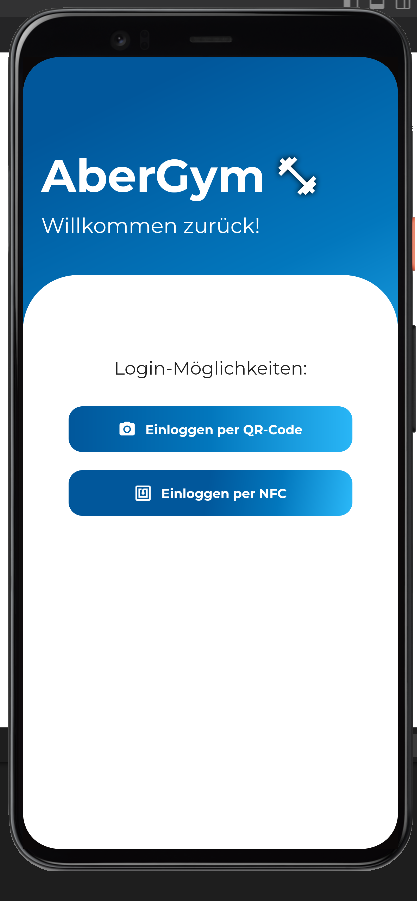
\includegraphics[scale=0.3]{pics/Start-Screen.png}
        \caption{Start-Screen}
    \end{figure}

Dieser wurde wie folgt implementiert:

\begin{lstlisting}[caption=Start-Screen Packages,label=lst:impl:frontend:packages]
    import 'package:abergymmobile/AGM.Animations/FadeAnimation.dart';
    import 'package:abergymmobile/AGM.Login/NFC.dart';
    import 'package:abergymmobile/AGM.Login/QrCode.dart';
    import 'package:google_fonts/google_fonts.dart';
    import 'package:flutter/foundation.dart';
    import 'package:flutter/material.dart';
    import 'package:flutter/services.dart';
\end{lstlisting}

Der Code importiert verschiedene Pakete, um das Layout und die Funktionen der Anwendung zu erstellen. Dazu gehören Google Fonts für benutzerdefinierte Schriftarten und Flutter-Pakete für Widgets und das Material Design.
\pagebreak

\begin{lstlisting}[caption= main-Funktion,label=lst:impl:frontend:main]
    Future<void> main() async {
        WidgetsFlutterBinding.ensureInitialized();
        SystemChrome.setEnabledSystemUIMode(SystemUiMode.manual, overlays: []);
        debugDefaultTargetPlatformOverride = null;
        runApp(const MaterialApp(
        debugShowCheckedModeBanner: false,
        home: LoginPage(),
        ));
        }
\end{lstlisting}

Die main-Funktion initialisiert die Flutter-App und startet sie. Sie setzt den System-UI-Modus und entfernt das Debug-Banner. Schließlich wird die LoginPage als Startseite festgelegt.
\newline

\begin{lstlisting}[caption=Login-Seite,label=lst:impl:frontend:login-seite]
    class LoginPage extends StatelessWidget {
const LoginPage({super.key});

@override
Widget build(BuildContext context) {
return Scaffold(
...
);
}
}
\end{lstlisting}

Das LoginPage-Widget erstellt die Login-Seite. Diese Seite ist in mehrere Abschnitte unterteilt, die im Folgenden erläutert werden.
\newline

\begin{lstlisting}[caption=Layout und Hintergrundfarbe,label=lst:impl:frontend:layout]
    decoration: BoxDecoration(
        gradient: LinearGradient(
        begin: Alignment.topCenter,
        colors: [
        Colors.lightBlue[900]!,
        Colors.lightBlue[800]!,
        Colors.lightBlue[400]!,
        ],
        ),
        ),
\end{lstlisting}

Mit LinearGradient wird ein linearer Farbverlauf von Hellblau bis Dunkelblau erstellt der von oben nach unten verläuft(begin: Allignment.topCenter).
\pagebreak

\begin{lstlisting}[caption=Logo und Willkommensnachricht,label=lst:impl:frontend:layout]
    children: <Widget>[
        FadeAnimation(
          1,
          Row(
            children: <Widget>[
              Text(
                "AberGym",
                style: GoogleFonts.montserrat(
                  color: Colors.white,
                  fontSize: 50,
                  fontWeight: FontWeight.bold,
                ),
              ),
              const SizedBox(width: 10),
              const Icon(
                Icons.fitness_center,
                color: Colors.white,
                size: 50,
                shadows: <Shadow>[
                  Shadow(
                    color: Colors.black,
                    blurRadius: 20.0,
                  )
                ],
              )
            ],
          ),
        ),
        const SizedBox(height: 10),
        FadeAnimation(
          1.3,
          Text(
            "Willkommen zurueck!",
            style: GoogleFonts.montserrat(
              color: Colors.white,
              fontSize: 23,
            ),
          ),
        ),
      ],
\end{lstlisting}

Der Code erstellt das AberGym-Logo und die Willkommensnachricht mit Hilfe von \texttt{FadeAnimation}, \texttt{Text}- und \texttt{Icon}-Widgets.
\pagebreak

\begin{lstlisting}[caption=QR-Code Schaltfläche,label=lst:impl:frontend:qrcode]
FadeAnimation(
1.6,
GestureDetector(
onTap: () {
Navigator.push(
context,
MaterialPageRoute(
builder: (context) => const QRCodePage(),
),
);
},
child: Container(
height: 50,
margin: const EdgeInsets.symmetric(horizontal: 20),
decoration: BoxDecoration(
gradient: LinearGradient(
begin: Alignment.centerLeft,
colors: [
Colors.lightBlue[900]!,
Colors.lightBlue[800]!,
Colors.lightBlue[400]!,
],
),
color: Colors.lightBlue,
borderRadius: BorderRadius.circular(15),
),
child: Row(
mainAxisAlignment: MainAxisAlignment.center,
children: [
const Icon(
Icons.camera_alt,
color: Colors.white,
size: 20,
),
const SizedBox(width: 10),
Text(
"Einloggen per QR-Code",
style: GoogleFonts.montserrat(
color: Colors.white,
fontWeight: FontWeight.bold,
),
),
],
),
),
),
),
\end{lstlisting}

Diese Schaltfläche ermöglicht dem Benutzer*der Benutzerin, sich per QR-Code einzuloggen. Sie verwendet \texttt{FadeAnimation}, \texttt{GestureDetector}, \texttt{Container} und \texttt{Row}-Widgets, um das Layout und die Funktionen der Schaltfläche zu erstellen. Beim Tippen auf die Schaltfläche wird der Benutzer*die Benutzerin zur \texttt{QRCodePage} weitergeleitet.
\pagebreak

\begin{lstlisting}[caption=NFC Schaltfläche,label=lst:impl:frontend:qrcode]
FadeAnimation(
1.7,
GestureDetector(
onTap: () {
Navigator.push(
context,
MaterialPageRoute(
builder: (context) => const NFC(),
),
);
},
child: Container(
height: 50,
margin: const EdgeInsets.symmetric(horizontal: 20),
decoration: BoxDecoration(
gradient: LinearGradient(
begin: Alignment.topCenter,
colors: [
Colors.lightBlue[900]!,
Colors.lightBlue[800]!,
Colors.lightBlue[400]!,
],
),
color: Colors.lightBlue,
borderRadius: BorderRadius.circular(15),
),
child: Row(
mainAxisAlignment: MainAxisAlignment.center,
children: [
const Icon(
Icons.nfc,
color: Colors.white,
size: 20,
),
const SizedBox(width: 10),
Text(
"Einloggen per NFC",
style: GoogleFonts.montserrat(
color: Colors.white,
fontWeight: FontWeight.bold,
),
),
],
),
),
),
),
\end{lstlisting}

Diese Schaltfläche ermöglicht dem Benutzer*der Benutzerin, sich per NFC einzuloggen. 
Ähnlich wie bei der QR-Code-Schaltfläche verwendet sie \texttt{FadeAnimation}, \texttt{GestureDetector}, \texttt{Container} und \texttt{Row}-Widgets, 
um das Layout und die Funktionen der Schaltfläche zu erstellen. Beim Tippen auf die Schaltfläche wird der Benutzer*die Benutzerin zur \texttt{NFC}-Seite weitergeleitet.
\newpage

\section{Login}
Um sich einzuloggen gibt es zwei Varianten. Entweder man loggt sich mithilfe eines QR-Codes ein oder mit NFC.

\subsection{QR-Code Login}

Die QR-Code-Funktion ermöglicht es Benutzer*innen, sich mit einem personalisierten QR-Code einzuloggen.

\begin{figure}[H]
    \centering
    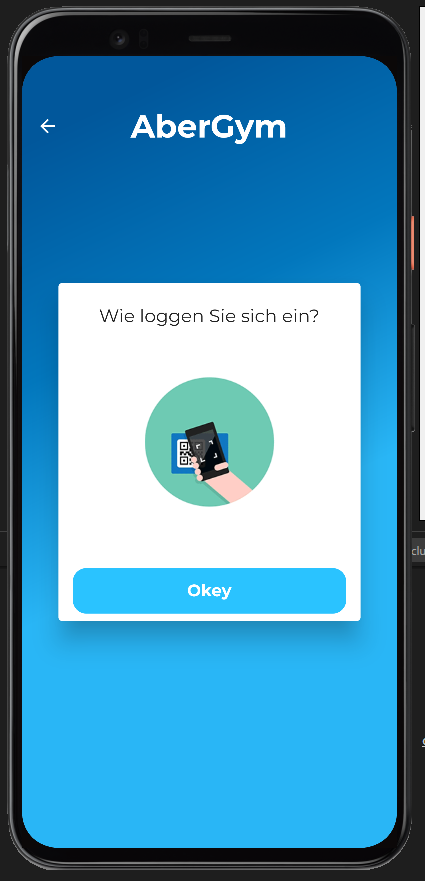
\includegraphics[scale=0.3]{pics/QRCodetutorial.png}
    \caption{QR-CodeTutorial}
\end{figure}
\begin{figure}[H]
    \centering
    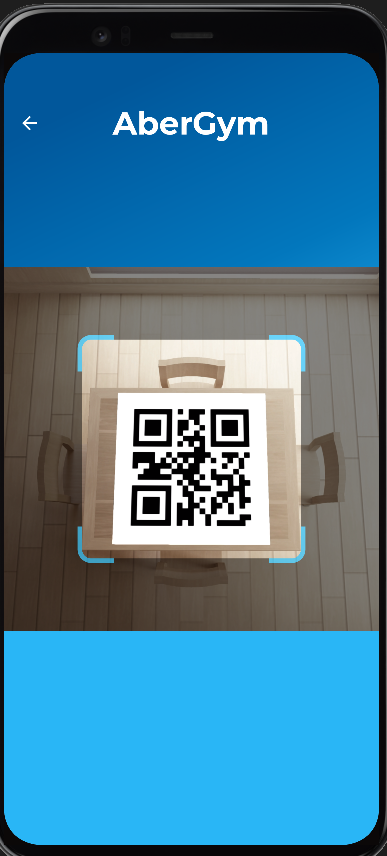
\includegraphics[scale=0.3]{pics/QR-CodeCamera.png}
    \caption{QR-Code auf Kamera}
\end{figure}
\pagebreak
\begin{lstlisting}[caption=QR-Code Seite erstellen,label=lst:impl:frontend:qrcode]
import 'package:qr_code_scanner/qr_code_scanner.dart';
import 'package:shared_preferences/shared_preferences.dart';

class QRCodePage extends StatefulWidget {
const QRCodePage({super.key});

@override
State<QRCodePage> createState() => _QRCodePageState();
}

class _QRCodePageState extends State<QRCodePage> {
final Color darkgrey = const Color.fromRGBO(37, 37, 50, 1);
final Color lightblue = const Color.fromARGB(255, 42, 195, 255);
bool showScanRect = false;
final GlobalKey qrKey = GlobalKey(debugLabel: 'QR');
Barcode? result;
QRViewController? controller;
bool logintrue = false;
String name = "";
bool _shouldNavigate = false;
\end{lstlisting}

Der Code beginnt mit dem Importieren der erforderlichen Pakete und dem Erstellen der \texttt{QRCodePage} StatefulWidget-Klasse. Der Zustand der Seite wird in der \texttt{QRCodePageState} Klasse verwaltet. Hier werden einige Variablen deklariert, wie zum Beispiel Farben, Zustände und der QRViewController.



\pagebreak
\begin{lstlisting}[caption=QR-Code Seitenstruktur,label=lst:impl:frontend:qrcode]
@override
Widget build(BuildContext context) {
return Scaffold(
extendBodyBehindAppBar: true,
appBar: AppBar(
title: Text(
'AberGym',
style: GoogleFonts.montserrat(
fontSize: 35,
color: Colors.white,
fontWeight: FontWeight.bold,
),
),
backgroundColor: Colors.transparent,
centerTitle: true,
elevation: 0,
),
body: Container(
width: double.infinity,
decoration: BoxDecoration(
gradient: LinearGradient(
begin: Alignment.topCenter,
colors: [
Colors.lightBlue[900]!,
Colors.lightBlue[800]!,
Colors.lightBlue[400]!,
],
),
),
child: Column(
mainAxisAlignment: MainAxisAlignment.center,
children: [
!showScanRect
? AlertDialog(
title: Text('Wie loggen Sie sich ein?',
textAlign: TextAlign.center,
style: GoogleFonts.getFont('Montserrat')),
content: Image.asset('assets/images/qrcode.gif'),
actions: [
GestureDetector(
child: Center(
child: Container(
width: 300,
height: 50,
decoration: BoxDecoration(
color: const Color.fromARGB(255, 42, 195, 255),
borderRadius: BorderRadius.circular(15),
),
child: Row(
mainAxisAlignment: MainAxisAlignment.center,
children: [
Text(
'Okey',
style: GoogleFonts.montserrat(
fontSize: 18,
color: Colors.white,
fontWeight: FontWeight.bold,
),
),
],
),
),
),
onTap: () {
setState(() {
showScanRect = true;
});
},
),
],
)
: SizedBox(
height: 400,
width: double.infinity,
child: _buildQrView(context),
),
],
),
),
);
}
\end{lstlisting}

In der \texttt{build}-Methode wird die Seitenstruktur der \texttt{QRCodePage} erstellt. Hier wird ein \texttt{Scaffold}-Widget verwendet, um die Hauptstruktur der Seite zu erzeugen. In der Mitte der Seite wird eine Bedingung geprüft, um entweder einen AlertDialog anzuzeigen, der Benutzer*innen darüber informiert, wie sie sich einloggen können, oder den QR-Code-Scanner anzuzeigen.
\linebreak
\begin{lstlisting}[caption=QR-Code Scanner erstellen,label=lst:impl:frontend:qrcode]
Widget _buildQrView(BuildContext context) {
var scanArea = (MediaQuery.of(context).size.width < 400 ||
MediaQuery.of(context).size.height < 400)
? 150.0
: 250.0;

return QRView(
key: qrKey,
onQRViewCreated: _onQRViewCreated,
overlay: QrScannerOverlayShape(
borderColor: lightblue,
borderRadius: 10,
borderLength: 30,
borderWidth: 10,
cutOutSize: scanArea),
);
}
\end{lstlisting}

Die \texttt{buildQrView}-Methode erstellt das QR-Code-Scanner-Widget. Das QRView-Widget erhält die Größe des Scanbereichs basierend auf der Bildschirmgröße und erstellt das Widget mit den angegebenen Design-Parametern.

\begin{lstlisting}[caption=QR-Code-Scanner Controller,label=lst:impl:frontend:qrcode]
void _onQRViewCreated(QRViewController controller) {
this.controller = controller;
controller.scannedDataStream.listen((scanData) {
setState(() {
result = scanData;
checkUser(result?.code);
});
if (_shouldNavigate) {
controller.dispose();
Navigator.of(context).pushReplacement(
MaterialPageRoute(builder: (context) => WelcomeSplashPage(name)));
}
});
}
\end{lstlisting}

Die \texttt{onQRViewCreated}-Methode wird aufgerufen, wenn das QRView-Widget erstellt wurde. Diese Methode initialisiert den \texttt{QRViewController} und hört auf den Datenstrom des gescannten QR-Codes. Wenn ein QR-Code gescannt wurde, wird die \texttt{checkUser} Methode aufgerufen, um die Benutzer*innen-Informationen abzurufen und die Seite zu navigieren, falls der Benutzer*die Benutzerin erfolgreich identifiziert wurde.

\begin{lstlisting}[caption=Datenbankabfrage QR-Code,label=lst:impl:frontend:qrcode]
Future<void> checkUser(String? qrCardId) async {
IResultSet result;

final conn = await MySQLConnection.createConnection(

);

await conn.connect();
result = await conn.execute(
"SELECT first_name, last_name FROM Person WHERE card_id = :card_id",
{"card_id": qrCardId},
);

for (final row in result.rows) {
setState(
() {
String? firstName = "";
String? lastName = "";
firstName = row.colAt(0);
lastName = row.colAt(1);
name = "$firstName $lastName";
},
);
}
final prefs = await SharedPreferences.getInstance();
if (name.isEmpty == false) {
setState(() {
_shouldNavigate = true;
logintrue = true;
prefs.setBool('login', logintrue);
prefs.setString('key', name);
});
}

await conn.close();
}
\end{lstlisting}

Die \texttt{checkUser}-Methode überprüft, ob der gescannte QR-Code mit einer gültigen Benutzerinnen-ID übereinstimmt, indem sie eine Datenbankabfrage durchführt. Sie verwendet die \texttt{MySQLConnection}-Klasse, um eine Verbindung zur Datenbank herzustellen, und führt eine SQL-Abfrage aus, um den Vornamen und Nachnamen des Benutzersin basierend auf der QR-Code-ID abzurufen. Wenn die Abfrage erfolgreich ist, wird der Name des Benutzers*in gespeichert und der Anmeldestatus in den \texttt{SharedPreferences} aktualisiert. Schließlich wird die Verbindung zur Datenbank geschlossen.

\pagebreak

\subsection{NFC Login}

Die NFC-Funktion ermöglicht es Benutzer*innen, sich mit einer Chipkarte wie einer Fitness-Mitgliedskarte einzuloggen.


\begin{lstlisting}[caption=NFC Package und State,label=lst:impl:frontend:qrcode]
import 'package:nfc_manager/nfc_manager.dart';

class NFC extends StatefulWidget {
const NFC({super.key});

@override
State<NFC> createState() => _NFCState();
}

class _NFCState extends State<NFC> {
bool _nfcEnabled = false;
ValueNotifier<dynamic> result = ValueNotifier(null);
final Color darkgrey = const Color.fromRGBO(37, 37, 50, 1);
final Color lightblue = const Color.fromARGB(255, 42, 195, 255);

@override
void initState() {
super.initState();
_checkNfcStatus();
}
}
\end{lstlisting}

Zunächst werden die erforderlichen Pakete importiert, insbesondere das \texttt{nfcmanager} Paket. Die \texttt{NFC}-Klasse erbt von \texttt{StatefulWidget}, und der zugehörige \texttt{State} wird in der \texttt{NFCState}-Klasse definiert. In \texttt{NFCState} werden die initialen Zustände und Farben gesetzt, und die Methode \texttt{initState} wird überschrieben, um den NFC-Status beim Start der Anwendung zu überprüfen.
\newline

\begin{lstlisting}[caption=NFC Status überprüfen,label=lst:impl:frontend:qrcode]
void _checkNfcStatus() async {
bool nfcEnabled = await NfcManager.instance.isAvailable();
setState(() {
_nfcEnabled = nfcEnabled;
});
}
\end{lstlisting}

Die Methode \texttt{checkNfcStatus} überprüft, ob NFC auf dem Gerät verfügbar und aktiviert ist. Mithilfe der \texttt{NfcManager}-Instanz wird die Methode \texttt{isAvailable} aufgerufen, um den NFC-Status abzurufen. Der ermittelte Status wird dann im \texttt{nfcEnabled} Attribut gespeichert.
\pagebreak

\begin{lstlisting}[caption=NFC Tag scannen,label=lst:impl:frontend:qrcode]
void _startScan() {
NfcManager.instance.startSession(onDiscovered: (NfcTag tag) async {
result.value = tag.data;
NfcManager.instance.stopSession();
});
}
\end{lstlisting}

Die Methode \texttt{startScan} startet die NFC-Session und wartet auf das Entdecken eines NFC-Tags. Sobald ein Tag entdeckt wird, wird die \texttt{onDiscovered}-Funktion aufgerufen, die die Daten des NFC-Tags in der \texttt{result}-Variable speichert und die Session beendet.
\newline
\begin{lstlisting}[caption=NFC Widget erstellen,label=lst:impl:frontend:qrcode]
    @override
    Widget build(BuildContext context) {
    return Scaffold(
    extendBodyBehindAppBar: true,
    appBar: AppBar(
    title: Text(
    'AberGym',
    style: GoogleFonts.montserrat(
    fontSize: 35,
    color: Colors.white,
    fontWeight: FontWeight.bold,
    ),
    ),
    backgroundColor: Colors.transparent,
    centerTitle: true,
    elevation: 0,
    ),
    backgroundColor: darkgrey,
    body: Container(
    decoration: BoxDecoration(
    gradient: LinearGradient(
    begin: Alignment.topCenter,
    colors: [
    Colors.lightBlue[900]!,
    Colors.lightBlue[800]!,
    Colors.lightBlue[400]!,
    ],
    ),
    ),
    child: _nfcEnabled
    ? Column(
    mainAxisAlignment: MainAxisAlignment.center,
    children: [
    Text(
    "Bitte halten Sie Ihre Fitnesskarte zum Handy, um die Karte zu scannen!",
    style: GoogleFonts.montserrat(
    color: Colors.white,
    fontWeight: FontWeight.bold,
    fontSize: 25,
    ),
    ),
    GestureDetector(
    onTap: _startScan,
    child: const Text("Karte scannen"),
    ),
    if (result.value != null) ...[Text(result.value)]
    ],
    )
    : Column(
    mainAxisAlignment: MainAxisAlignment.center,
    children: [
    Text(
    "Bitte schalten Sie NFC ein, um die Karte zu scannen!",
    style: GoogleFonts.montserrat(
    color: Colors.white,
    fontWeight: FontWeight.bold,
    fontSize: 25,
    ),
    textAlign: TextAlign.center,
    ),
    ],
    ),
    ),
    );
    }
    \end{lstlisting}
    
    In der \texttt{build}-Methode wird das Haupt-Widget der NFC-Seite erstellt. Ein \texttt{Scaffold}-Widget wird verwendet, um das grundlegende Layout der Seite zu definieren, einschließlich der AppBar und des Hintergrundfarbverlaufs. Im Hauptteil der Seite wird überprüft, ob NFC aktiviert ist. Wenn NFC aktiviert ist, wird der Benutzer*die Benutzerin aufgefordert, die Fitnesskarte zum Gerät zu halten, und ein GestureDetector-Widget erlaubt das Starten des Scanvorgangs. Andernfalls wird der Benutzer*die Benutzerin aufgefordert, NFC zu aktivieren.

    \begin{figure}[H]
        \centering
        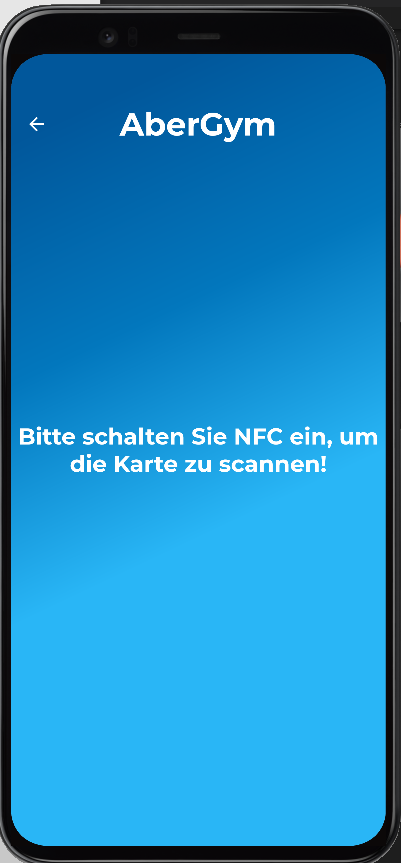
\includegraphics[scale=0.5]{pics/NFC.png}
        \caption{NFC}
    \end{figure}

    \newpage

    \section{Hauptmenü}
    \author{Antonio Kuvac}

    Im Hauptmenü kann der Benutzer*die Benutzerin sich den aktuellen Trainingsplan ansehen, den letzten Trainingsplan ansehen oder den Trainingsplan starten.

    \begin{figure}[H]
        \centering
        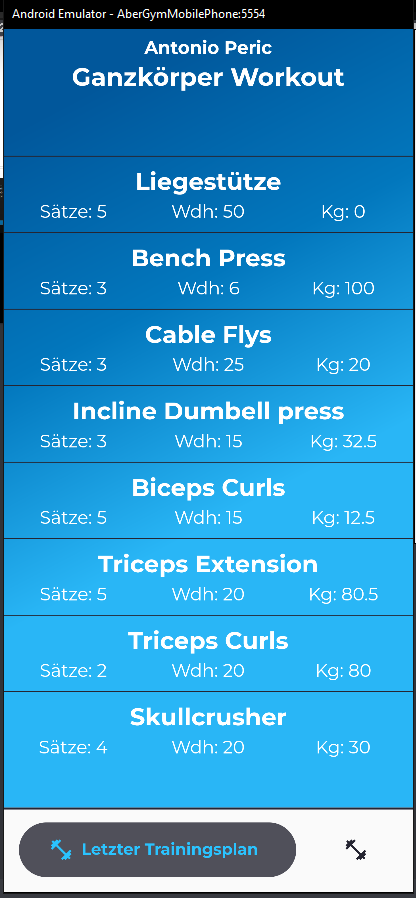
\includegraphics[scale=0.5]{pics/mainmenu.png}
        \caption{Hauptmenü}
    \end{figure}

    \pagebreak
    \subsection{Layout}


\begin{lstlisting}[caption=Layout Packages,label=lst:impl:frontend:qrcode]
import 'package:google_fonts/google_fonts.dart';
import 'package:google_nav_bar/google_nav_bar.dart';
\end{lstlisting}

Das Paket \texttt{googlefonts} ermöglicht die Verwendung von Google Fonts, während das Paket \texttt{googlenavbar} für die Erstellung der Navigationsleiste verwendet wird.
\\

\begin{lstlisting}[caption=LayoutState,label=lst:impl:frontend:qrcode]
class _LayoutState extends State<Layout> {
final bodies = [const SecondPage(), const HomePage()];
int currentIndex = 1;
Color lightblue = const Color.fromARGB(255, 42, 195, 255);
Color darkgrey = const Color.fromRGBO(37, 37, 50, 1);
\end{lstlisting}

Die Klasse \texttt{LayoutState} erbt von der \texttt{State<Layout>} Basisklasse und definiert einige Eigenschaften, wie die Liste der Seiten, den aktuellen ausgewählten Index und Farben für das Design der Navigationsleiste.
\\

\begin{lstlisting}[caption=Layout Scaffold-Widget,label=lst:impl:frontend:qrcode]
@override
Widget build(BuildContext context) {
return Scaffold(
body: bodies[currentIndex],
bottomNavigationBar: Stack(
\end{lstlisting}

Das \texttt{Scaffold}-Widget stellt das Grundgerüst für das Layout der App bereit. Der \texttt{body} wird durch den aktuellen ausgewählten Index in der \texttt{bodies}-Liste bestimmt. Die \texttt{bottomNavigationBar} ist ein \texttt{Stack}-Widget, das die Navigationsleiste und eine Linie oben auf der Navigationsleiste enthält.
\\

\begin{lstlisting}[caption=Navbar,label=lst:impl:frontend:qrcode]
children: [
Padding(
padding: const EdgeInsets.symmetric(horizontal: 15.0, vertical: 15),
child: GNav(
curve: Curves.easeOutSine,
color: darkgrey,
gap: 8,
iconSize: 25,
activeColor: lightblue,
tabBackgroundColor: darkgrey.withOpacity(0.8),
padding: const EdgeInsets.symmetric(vertical: 15, horizontal: 30),
duration: const Duration(milliseconds: 500),
tabs: [
GButton(
icon: Icons.fitness_center,
text: "Letzter Trainingsplan",
textStyle: GoogleFonts.montserrat(
color: lightblue,
fontSize: 16,
fontWeight: FontWeight.bold,
),
),
GButton(
icon: Icons.fitness_center,
text: "Heutiger Trainingsplan",
textStyle: GoogleFonts.montserrat(
color: lightblue,
fontSize: 16,
fontWeight: FontWeight.bold,
),
),
],
selectedIndex: currentIndex,
onTabChange: (index) {
    setState(() {
    currentIndex = index;
    });
    },
    ),
    ),
    Positioned(
    top: 0,
    left: 0,
    right: 0,
    child: Container(
    height: 2,
    color: darkgrey,
    ),
    ),
    ],
    ),
    );
    }
    }
}
\end{lstlisting}
    
    Die \texttt{GNav}-Komponente erstellt die Navigationsleiste und definiert deren Aussehen und Verhalten. Die Navigationsleiste besteht aus zwei \texttt{GButton}-Widgets, die jeweils ein Icon und einen Text enthalten. Der Stil des Textes wird mit dem GoogleFonts-Paket festgelegt. Die \texttt{selectedIndex}-Eigenschaft gibt den ausgewählten Index der Navigationsleiste an, und die \texttt{onTabChange}-Eigenschaft ist eine Funktion, die den aktuellen Index aktualisiert, wenn der Benutzer*die Benutzerin eine andere Registerkarte auswählt.
    

    \subsection{HomePage}
    \author{Antonio Kuvac}

\begin{lstlisting}[caption=Trainingsplan Logik,label=lst:impl:frontend:qrcode]
final prefs = await SharedPreferences.getInstance();
int? amountrows = prefs.getInt('amountrows');
int countTrue = 0;

        if (amountrows != null) {
          for (int i = 0; i < amountrows; i++) {
            if (prefs.getBool('finishedExcersice_$i') == true) {
              countTrue++;
            }
          }
          if (countTrue == amountrows) {
            for (int i = 0; i < amountrows; i++) {
              prefs.remove('finishedExcersice_$i');
            }
          }
        }

        _navigateToNextScreen(context);
\end{lstlisting}

Innerhalb der \texttt{onPressed}-Funktion wird die Logik für das Starten des Trainingsplans und das Verwalten der SharedPreferences implementiert. Die SharedPreferences-Instanz wird abgerufen, und die Anzahl der Zeilen und die Anzahl der abgeschlossenen Übungen werden verwaltet. Wenn alle Übungen abgeschlossen sind, werden die SharedPreferences-Einträge entfernt. Schließlich wird die Funktion \texttt{navigateToNextScreen} aufgerufen, um zur nächsten Seite zu navigieren.
\\

\begin{lstlisting}[caption=Trainingsplan starten Knopf,label=lst:impl:frontend:qrcode]
style: ElevatedButton.styleFrom(
backgroundColor: darkgrey.withOpacity(0.8),
shape: const RoundedRectangleBorder(
borderRadius: BorderRadius.only(
topRight: Radius.circular(0.0),
topLeft: Radius.circular(0.0),
),
),
),
child: SizedBox(
height: 216,
child: Column(
),
),
\end{lstlisting}

Für den Trainingsplan Starten Knopf wurde der Hintergrund des \texttt{ElevatedButton}-Widgets mit einer leicht transparenten dunkelgrauen Farbe festgelegt. Die Form des Buttons ist ein rechteckiges Widget mit abgerundeten Ecken an der Oberseite. Der Inhalt des Buttons besteht aus einer \texttt{SizedBox} mit einer festen Höhe und einer \texttt{Column}, die die Text- und Icon-Widgets enthält.
\\


\begin{lstlisting}[caption=HomePage Navigation,label=lst:impl:frontend:qrcode]
void _navigateToNextScreen(BuildContext context) {
Navigator.of(context)
.push(MaterialPageRoute(builder: (context) => const LayoutTDL()));
}
\end{lstlisting}

Die Navigationsfunktion \texttt{navigateToNextScreen} wird definiert, um zur nächsten Seite zu navigieren.Die Funktion \texttt{navigateToNextScreen} akzeptiert ein \texttt{BuildContext}-Objekt und verwendet den \texttt{Navigator} zum Navigieren zur nächsten Seite, die durch das \texttt{LayoutTDL}-Widget dargestellt wird.

\pagebreak
    \subsection{SecondPage}
    \author{Antonio Kuvac}

    \begin{lstlisting}[caption=Second Page,label=lst:impl:frontend:qrcode]
        class SecondPage extends StatelessWidget {
  const SecondPage({super.key});

  @override
  Widget build(BuildContext context) {
    return SqlTable(version: 0);
  }
}
    \end{lstlisting}

    Die SecondPage Methode lädt, wenn die "Letzter Trainingsplan" Seite ausgewählt wird, aus der Datenbank den letzten Trainingsplan. 

    

    \section{To-Do-Liste}
    \author{Antonio Kuvac}

    Die To-Do-Liste ist eine interaktive Liste aus Übungen die im Trainingsplan enthalten sind. Durch das Auswählen einer Übung in dieser Liste, wird man an die Satzzähler Seite weitergeleitet. Wenn man eine Übung abgeschlossen hat, wird die Übung in der Liste ausgegraut und an letzter Stelle der Liste verschoben.

    \begin{figure}[H]
        \centering
        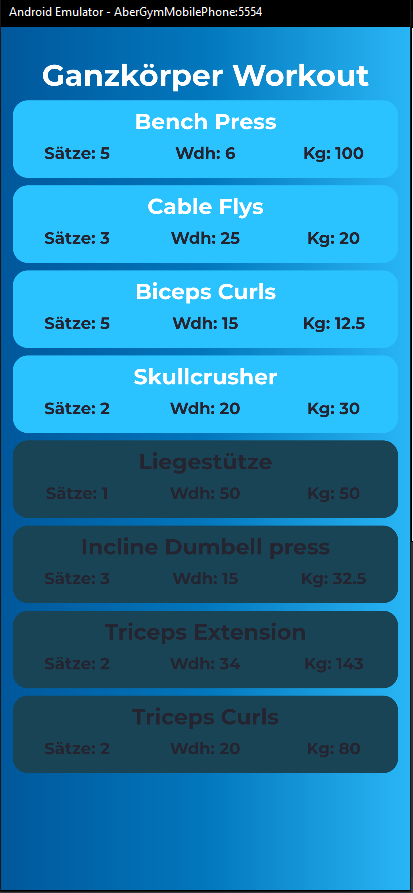
\includegraphics[scale=0.3]{pics/To-Do-Liste.png}
        \caption{To-Do-Liste}
    \end{figure}
    
    \pagebreak
    \begin{lstlisting}[caption=To-Do-Liste Trainingsplan Variablen,label=lst:impl:frontend:qrcode]
    late String wname = "";
    late List<String> wereps = [];
    late List<String> wesets = [];
    late List<String> weweight = [];
    late List<String> ename = [];
    late int amountrows = 0;
    final Color lightblue = const Color.fromARGB(255, 42, 195, 255);
    final Color darkgrey = const Color.fromRGBO(37, 37, 50, 1);
    List<bool> finishedExcersiceList = [];
    int counter = 0;
    bool finished = false;
    \end{lstlisting}
    
    Diese Variablen enthalten Informationen über die Übungen, die Anzahl der Zeilen, Farben und ob eine Übung abgeschlossen ist oder nicht.
    \\
    
    
    \begin{lstlisting}[caption=To-Do-Liste get Methode,label=lst:impl:frontend:qrcode]
        void getData() async {
            final prefs = await SharedPreferences.getInstance();
            wname = prefs.getString('wname')!;
            wereps = prefs.getStringList('wereps')!;
            wesets = prefs.getStringList('wesets')!;
            weweight = prefs.getStringList('weweight')!;
            ename = prefs.getStringList('ename')!;
            amountrows = prefs.getInt('amountrows')!;
        
            for (int i = 0; i < amountrows; i++) {
              if (prefs.get('finishedExcersice_$i') == true) {
                finishedExcersiceList.add(true);
                setState(() {
                  counter++;
                });
              } else {
                finishedExcersiceList.add(false);
              }
            }
            if (counter == amountrows) {
              setState(() {
                finished = true;
              });
            }
            setState(() {
              wname = wname;
              wereps = wereps;
              wesets = wesets;
              wesets = wesets;
              weweight = weweight;
              ename = ename;
              amountrows = amountrows;
            });
          }
    \end{lstlisting}
    
    Die Methode \texttt{getData} liest die Daten aus SharedPreferences und aktualisiert die Zustände der ToDoList-Klasse. 
    
    \pagebreak
    \begin{lstlisting}[caption=To-Do-Liste Item Methode,label=lst:impl:frontend:qrcode]
        Container toDoListItem(int i, bool isFinished) {
            return Container(
              height: 78,
              margin: const EdgeInsets.only(
                top: 3.8,
                right: 12,
                left: 12,
                bottom: 3.8,
              ),
              decoration: isFinished
                  ? BoxDecoration(
                      borderRadius: BorderRadius.circular(15.0),
                      color: const Color.fromARGB(255, 25, 68, 85),
                    )
                  : BoxDecoration(
                      borderRadius: BorderRadius.circular(15.0),
                      color: lightblue,
                    ),
              child: Column(
                children: [
                  Container(
                    padding: const EdgeInsets.all(8.0),
                    child: Text(
                      (ename.isNotEmpty ? ename[i].toString() : ""),
                      textScaleFactor: 2,
                      style: isFinished
                          ? GoogleFonts.montserrat(
                              fontSize: 11,
                              color: darkgrey,
                              fontWeight: FontWeight.bold,
                            )
                          : GoogleFonts.montserrat(
                              fontSize: 11,
                              color: Colors.white,
                              fontWeight: FontWeight.bold,
                            ),
                      textAlign: TextAlign.center,
                    ),
                  ),
                  Table(
                    children: [
                      TableRow(
                        children: [
                          Center(
                            child: Text(
                              (wesets.isNotEmpty
                                  ? 'Saetze: ${wesets[i].toString()}'
                                  : ""),
                              textScaleFactor: 1.5,
                              style: GoogleFonts.montserrat(
                                fontSize: 11,
                                color: darkgrey,
                                fontWeight: FontWeight.bold,
                              ),
                            ),
                          ),
                          Center(
                            child: Text(
                              (wereps.isNotEmpty ? 'Wdh: ${wereps[i].toString()}' : ""),
                              textScaleFactor: 1.5,
                              style: GoogleFonts.montserrat(
                                fontSize: 11,
                                color: darkgrey,
                                fontWeight: FontWeight.bold,
                              ),
                            ),
                          ),
                          Center(
                            child: Text(
                              (weweight.isNotEmpty
                                  ? 'Kg: ${weweight[i].toString()}'
                                  : ""),
                              textScaleFactor: 1.5,
                              style: GoogleFonts.montserrat(
                                fontSize: 11,
                                color: darkgrey,
                                fontWeight: FontWeight.bold,
                              ),
                            ),
                          ),
                        ],
                      ),
                    ],
                  ),
                ],
              ),
            );
          }
        
    \end{lstlisting}

    Die \texttt{toDoListItem}-Methode erstellt ein individuelles Aufgabenlisten-Element basierend auf einem gegebenen Index und ob es abgeschlossen ist oder nicht.

    \section{Satzzähler}
    \author{Antonio Kuvac}

    Der Satzzähler ermöglicht es beim Trainieren, die Sätze der aktuell ausgewählten Übung mitzuzählen und somit die Übung abzuschließen.

    \begin{figure}[H]
        \centering
        \includegraphics[scale=0.3]{pics/Satzzähler.png}
        \caption{Satzzähler}
    \end{figure}

    \begin{lstlisting}[caption=SetCounter,label=lst:impl:frontend:qrcode]
        class SetCounter extends StatefulWidget {
        int index = 0;
        SetCounter({super.key, required this.index});
        
        @override
        State<SetCounter> createState() => _SetCounterState(index);
        }
        \end{lstlisting}
        
        Die Klasse SetCounter erbt von StatefulWidget und nimmt den Parameter index entgegen. Dieser Index gibt die Position der aktuellen Übung in der Liste an. Der Konstruktor der Klasse speichert den Index und übergibt ihn an den State der Klasse, SetCounterState.
        \\
        
        \begin{lstlisting}[caption=SetCounterState,label=lst:impl:frontend:qrcode]
        class _SetCounterState extends State<SetCounter> {
        int index = 0;
        late List<String> werepsList = [];
        late List<String> wesetsList = [];
        late List<String> weweightList = [];
        late List<String> enameList = [];
        String wereps = "";
        String wesets = "";
        String weweight = "";
        String ename = "";
        Color lightblue = const Color.fromARGB(255, 42, 195, 255);
        Color darkgrey = const Color.fromRGBO(37, 37, 50, 1);
        int counter = 0;
        late bool finishedExcersice;
        double? fontSizeRows = 13;
        double? fontPixelsRows = 1.5;
        
        _SetCounterState(this.index);
        }
        \end{lstlisting}
        
        Die Klasse SetCounterState speichert den index und verwaltet die Zustände der App. Es gibt verschiedene Zustandsvariablen für die Anzahl der Wiederholungen, Sätze, das Gewicht und den Namen der Übung. 
        \\
        
        
        \begin{lstlisting}[caption=Increase Counter Funktion,label=lst:impl:frontend:qrcode]
        void increaseCounter() async {
        final prefs = await SharedPreferences.getInstance();
        setState(() => counter++);
        if (counter > int.parse(wesets)) {
        finishedExcersice = true;
        prefs.setBool('finishedExcersice$index', finishedExcersice);
        }
        }
        \end{lstlisting}

        Die increaseCounter-Funktion erhöht den Satzzähler und aktualisiert die Benutzeroberfläche. Wenn die Anzahl der abgeschlossenen Sätze größer ist als die vorgegebene Anzahl der Sätze, wird die Variable finishedExcersice auf true gesetzt und in den SharedPreferences gespeichert.
        \\

        \begin{lstlisting}[caption=initState,label=lst:impl:frontend:qrcode]
            @override
            void initState() {
            super.initState();
            getData();
            }
            \end{lstlisting}
            \pagebreak
            Die initState()-Funktion wird aufgerufen, wenn der Zustand des Widgets initialisiert wird. Hier wird die Funktion getData() aufgerufen, um die Daten für die aktuelle Übung zu laden.
            \\
            
            \begin{lstlisting}[caption=GestureDetector,label=lst:impl:frontend:qrcode]
                GestureDetector(
                    onTap: _increaseCounter,
                    child: Container(
                      padding: const EdgeInsets.only(top: 65),
                      margin: const EdgeInsets.all(50.0),
                      width: 300.0,
                      height: 300.0,
                      decoration: BoxDecoration(
                        gradient: LinearGradient(
                          begin: Alignment.centerLeft,
                          colors: [
                            Colors.lightBlue[900]!,
                            Colors.lightBlue[800]!,
                            Colors.lightBlue[400]!,
                          ],
                        ),
                        shape: BoxShape.circle,
                      ),
                      child: Column(
                        children: [
                          Text(
                            '$counter/$wesets',
                            style: GoogleFonts.montserrat(
                              color: Colors.white,
                              fontSize: 100,
                            ),
                          ),
                          Text(
                            "Erledigte Saetze",
                            style: GoogleFonts.montserrat(
                              color: Colors.white,
                              fontSize: 25,
                              fontWeight: FontWeight.bold,
                            ),
                          ),
                        ],
                      ),
                    ),
                  ),
            \end{lstlisting}
            
            Ein GestureDetector wird verwendet, um auf Berührungen des Benutzers zu reagieren und den Satzzähler entsprechend zu erhöhen. Wenn der Benutzer auf den Container tippt, wird die increaseCounter-Funktion aufgerufen.
            \\

            \begin{lstlisting}[caption=GestureDetector zum Schluss,label=lst:impl:frontend:qrcode]
                GestureDetector(
                    onTap: () {
                      Navigator.push(
                        context,
                        MaterialPageRoute(
                          builder: (context) => const ToDoList(),
                        ),
                      );
                    },
                    child: Container(
                      padding: const EdgeInsets.only(top: 65),
                      margin: const EdgeInsets.all(50.0),
                      width: 300.0,
                      height: 300.0,
                      decoration: BoxDecoration(
                        gradient: LinearGradient(
                          begin: Alignment.centerLeft,
                          colors: [
                            Colors.lightBlue[900]!,
                            Colors.lightBlue[800]!,
                            Colors.lightBlue[400]!,
                          ],
                        ),
                        shape: BoxShape.circle,
                      ),
                      child: Column(
                        children: [
                          InkWell(
                            onTap: () {
                              Navigator.push(
                                context,
                                MaterialPageRoute(
                                  builder: (context) => const ToDoList(),
                                ),
                              );
                            },
                            child: Column(
                              children: <Widget>[
                                Text(
                                  "Uebung",
                                  style: GoogleFonts.montserrat(
                                    color: Colors.white,
                                    fontSize: 70,
                                  ),
                                ),
                                Text(
                                  "Fertig",
                                  style: GoogleFonts.montserrat(
                                    color: Colors.white,
                                    fontSize: 65,
                                  ),
                                ),
                              ],
                            ),
                          ),
                        ],
                      ),
                    ),
                  ),
            \end{lstlisting}
            
            Wenn die Übung abgeschlossen ist (wenn die Anzahl der abgeschlossenen Sätze gleich oder größer als die vorgegebene Anzahl ist), wird ein anderer GestureDetector und Container angezeigt, der dem Benutzer signalisiert, dass die Übung beendet ist. Bei einem Tippen auf den Container wird der Benutzer zur ToDoList-Seite weitergeleitet.
            \\

    \section{Trainingplan bearbeiten}
    \author{Antonio Kuvac}

    Durch langes gedrückt halten einer Übung in der To-Do-Liste wird die Bearbeitungsseite geöffnet und die ausgewählte Übung kann bearbeitet werden. Es können die Wiederholungen, die Sätze und das Gewicht geändert werden, um während des Trainings flexibel auf eigene Wünsche das Training anpassen zu können.

    \begin{figure}[H]
        \centering
        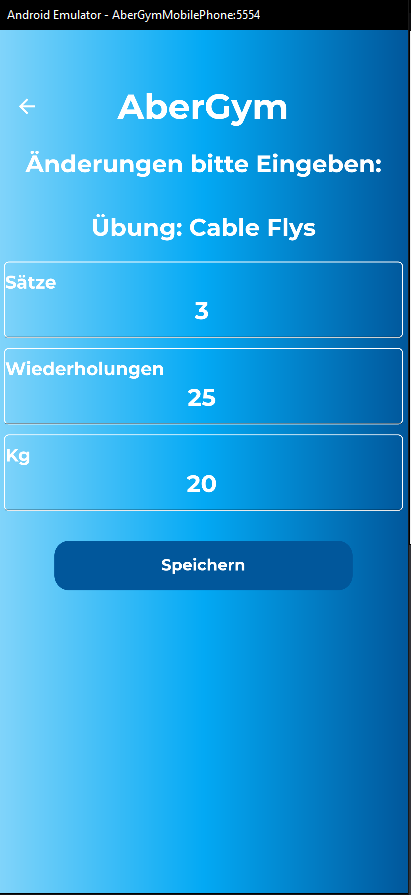
\includegraphics[scale=0.3]{pics/Bearbeiten.png}
        \caption{Trainingplan bearbeiten}
    \end{figure}

    \begin{lstlisting}[caption=Bearbeiten Index,label=lst:impl:frontend:qrcode]
        class UpdateExcersice extends StatefulWidget {
        int index = 0;
        UpdateExcersice({super.key, required this.index});
        
        @override
        State<UpdateExcersice> createState() => _UpdateExcersiceState(index);
        }
        \end{lstlisting}
        
        Die UpdateExcersice-Klasse erbt von StatefulWidget und speichert den index der aktuellen Übung. Der Konstruktor nimmt den index als erforderliches Argument an und übergibt diesen an die UpdateExcersiceState-Klasse.
        \\
         

        \begin{lstlisting}[caption=Bearbeiten UpdateExcersiceState,label=lst:impl:frontend:qrcode]
              class _UpdateExcersiceState extends State<UpdateExcersice> {
                int index = 0;
                late List<String> werepsList = [];
                late List<String> wesetsList = [];
                late List<String> weweightList = [];
                late List<String> enameList = [];
                String wereps = "";
                String wesets = "";
                String weweight = "";
                String ename = "";
                Color lightblue = const Color.fromARGB(255, 42, 195, 255);
                Color darkgrey = const Color.fromRGBO(37, 37, 50, 1);
                String _sets = '';
                String _reps = '';
                String _kg = '';
                final setsController = TextEditingController();
                final repsController = TextEditingController();
                final kgController = TextEditingController();
              
                _UpdateExcersiceState(this.index);
              
                void getData() async {
                  final prefs = await SharedPreferences.getInstance();
                  werepsList = prefs.getStringList('wereps')!;
                  wesetsList = prefs.getStringList('wesets')!;
                  weweightList = prefs.getStringList('weweight')!;
                  enameList = prefs.getStringList('ename')!;
              
                  setState(() {
                    wereps = werepsList[index];
                    wesets = wesetsList[index];
                    weweight = weweightList[index];
                    ename = enameList[index];
                    setsController.text = wesets;
                    repsController.text = wereps;
                    kgController.text = weweight;
                  });
                }}
        \end{lstlisting}
        
        Die UpdateExcersiceState-Klasse erweitert die State-Klasse für das UpdateExcersice-Widget. Innerhalb dieser Klasse werden verschiedene Variablen und Methoden definiert, um Daten zu laden, zu speichern und die Benutzeroberfläche aufzubauen.
        \\
        

        \begin{lstlisting}[caption=Bearbeiten initState getData,label=lst:impl:frontend:qrcode]
        void initState() {
        super.initState();
        getData();
        }
        \end{lstlisting}
        
        Die initState-Methode wird aufgerufen, wenn der Zustand des Widgets initialisiert wird. Hier wird die getData-Methode aufgerufen, um die aktuellen Daten der Übung zu laden.
        \\

        \begin{lstlisting}[caption=Bearbeiten Build,label=lst:impl:frontend:qrcode]
        @override
        Widget build(BuildContext context) {
            @override
            Widget build(BuildContext context) {
              return Scaffold(
                extendBodyBehindAppBar: true,
                appBar: AppBar(
                  title: Text(
                    'AberGym',
                    style: GoogleFonts.montserrat(
                      fontSize: 35,
                      color: Colors.white,
                      fontWeight: FontWeight.bold,
                    ),
                  ),
                  backgroundColor: Colors.transparent,
                  centerTitle: true,
                  elevation: 0,
                ),
                body: Container(
                  padding: const EdgeInsets.only(top: 110),
                  decoration: BoxDecoration(
                    gradient: LinearGradient(
                      begin: Alignment.centerLeft,
                      colors: [
                        Colors.lightBlue[200]!,
                        Colors.lightBlue[500]!,
                        Colors.lightBlue[900]!,
                      ],
                    ),
                  ),
                  child: Center(
                    child: Column(
                      children: [
                        Container(
                          padding: const EdgeInsets.all(10.0),
                          child: Text(
                            "Aenderungen bitte Eingeben:",
                            style: GoogleFonts.montserrat(
                              fontSize: 24,
                              color: Colors.white,
                              fontWeight: FontWeight.bold,
                            ),
                            textAlign: TextAlign.center,
                          ),
                        ),
                        Container(
                          padding: const EdgeInsets.only(bottom: 15.0, top: 25),
                          child: Text(
                            'Uebung: $ename',
                            style: GoogleFonts.montserrat(
                              fontSize: 24,
                              color: Colors.white,
                              fontWeight: FontWeight.bold,
                            ),
                            textAlign: TextAlign.center,
                          ),
                        ),
                        // Textfeld 1
                        Container(
                          margin: const EdgeInsets.all(5),
                          decoration: BoxDecoration(
                            borderRadius: BorderRadius.circular(5),
                            border: Border.all(color: Colors.white),
                          ),
                          child: TextField(
                            keyboardType: TextInputType.number,
                            decoration: InputDecoration(
                              labelText: 'Saetze',
                              labelStyle: GoogleFonts.montserrat(
                                fontSize: 24,
                                color: Colors.white,
                                fontWeight: FontWeight.bold,
                              ),
                            ),
                            controller: setsController,
                            onChanged: (value) {
                              _saveInput();
                            },
                            onTap: () {
                              setsController.clear();
                            },
                            textAlign: TextAlign.center,
                            style: GoogleFonts.montserrat(
                              fontSize: 24,
                              color: Colors.white,
                              fontWeight: FontWeight.bold,
                            ),
                          ),
                        ),
                        // Textfeld 2
                        Container(
                          margin: const EdgeInsets.all(5),
                          decoration: BoxDecoration(
                            borderRadius: BorderRadius.circular(5),
                            border: Border.all(color: Colors.white),
                          ),
                          child: TextField(
                            keyboardType: TextInputType.number,
                            decoration: InputDecoration(
                              labelText: 'Wiederholungen',
                              labelStyle: GoogleFonts.montserrat(
                                fontSize: 24,
                                color: Colors.white,
                                fontWeight: FontWeight.bold,
                              ),
                            ),
                            controller: repsController,
                            onChanged: (value) {
                              _saveInput();
                            },
                            onTap: () {
                              repsController.clear();
                            },
                            textAlign: TextAlign.center,
                            style: GoogleFonts.montserrat(
                              fontSize: 24,
                              color: Colors.white,
                              fontWeight: FontWeight.bold,
                            ),
                          ),
                        ),
                        // Textfeld 3
                        Container(
                          margin: const EdgeInsets.all(5),
                          decoration: BoxDecoration(
                            borderRadius: BorderRadius.circular(5),
                            border: Border.all(color: Colors.white),
                          ),
                          child: TextField(
                            keyboardType: TextInputType.number,
                            decoration: InputDecoration(
                              labelText: 'Kg',
                              labelStyle: GoogleFonts.montserrat(
                                fontSize: 24,
                                color: Colors.white,
                                fontWeight: FontWeight.bold,
                              ),
                            ),
                            controller: kgController,
                            onChanged: (value) {
                              _saveInput();
                            },
                            onTap: () {
                              kgController.clear();
                            },
                            textAlign: TextAlign.center,
                            style: GoogleFonts.montserrat(
                              fontSize: 24,
                              color: Colors.white,
                              fontWeight: FontWeight.bold,
                            ),
                          ),
                        ),
                        GestureDetector(
                          onTap: () async {
                            await saveInputInCache();
                            Navigator.push(
                              context,
                              PageTransition(
                                type: PageTransitionType.leftToRight,
                                child: const LayoutTDL(),
                              ),
                            );
                          },
                          child: Container(
                            margin: const EdgeInsets.only(top: 25),
                            width: 300,
                            height: 50,
                            decoration: BoxDecoration(
                              color: Colors.lightBlue[900]!,
                              borderRadius: BorderRadius.circular(15),
                            ),
                            child: Row(
                              mainAxisAlignment: MainAxisAlignment.center,
                              children: [
                                Text(
                                  'Speichern',
                                  style: GoogleFonts.montserrat(
                                    fontSize: 16,
                                    color: Colors.white,
                                    fontWeight: FontWeight.bold,
                                  ),
                                ),
                              ],
                            ),
                          ),
                        ),
                      ],
                    ),
                  ),
                ),
              );
            }
        }
        \end{lstlisting}
        
        Die build-Methode erstellt die Benutzeroberfläche für das Widget. In dieser Methode wird ein Scaffold-Widget verwendet, um die grundlegende Struktur der App zu definieren. Die Benutzeroberfläche besteht aus mehreren Eingabefeldern und Schaltflächen, die den Benutzer*innen ermöglichen, ihre Änderungen einzugeben und zu speichern.
        \\
        

        \begin{lstlisting}[caption=Bearbeiten saveInput,label=lst:impl:frontend:qrcode]
        void _saveInput() {
        setState(() {
        _sets = setsController.text;
        _reps = repsController.text;
        _kg = kgController.text;
        });
        }
        \end{lstlisting}
        
        Die saveInput-Methode speichert die Benutzereingaben in den entsprechenden Variablen. Diese Methode wird aufgerufen, wenn der Inhalt eines der Eingabefelder geändert wird.
        \\
        

        \begin{lstlisting}[caption=Bearbeiten saveInputInCache,label=lst:impl:frontend:qrcode]
            Future<void> saveInputInCache() async {
                  await conn.connect();
                  await conn.execute(
                    'UPDATE WorkoutExercise we JOIN Exercise e ON we.exercise_id = e.id SET we.`sets` = :sets, we.weight = :kg, we.reps = :reps WHERE e.name = :name AND we.workoutplan_id = (SELECT MAX(id) FROM Workoutplan)',
                    {"sets": _sets, "kg": _kg, "reps": _reps, "name": ename},
                  );
                  wesetsList[index] = _sets;
                  weweightList[index] = _kg;
                  werepsList[index] = _reps;
                  final prefs = await SharedPreferences.getInstance();
            
                  await prefs.remove('wesets');
                  await prefs.remove('weweight');
                  await prefs.remove('wereps');
            
                  await prefs.setStringList('wesets', wesetsList);
                  await prefs.setStringList('weweight', weweightList);
                  await prefs.setStringList('wereps', werepsList);
            
                  conn.close();
                }
        \end{lstlisting}
        
        Die saveInputInCache-Methode speichert die Benutzereingaben in den SharedPreferences und aktualisiert die Datenbank. Diese Methode wird aufgerufen, wenn der*die Benutzer*innen auf die Schaltfläche ``Speichern'' tippt.	

\begin{spacing}{1}
\chapter{Backend}\label{chapter:backend}
\end{spacing}
\section{Temporäres Backend für die Mobile Anwendung}
\setauthor{Antonio Peric}

\subsection{IntelliJ Projekt}
\setauthor{Antonio Peric} 
In der vorliegenden Arbeit wurde ein temporäres Backend mithilfe der Technologieumgebung IntelliJ \cite{Quarkus} und der Programmiersprache Java  \cite{Java} entwickelt. Bei der Umsetzung wurde besonderes Augenmerk auf eine präzise Definition der einzelnen Entitäten, eine klare Setzung der Attribute sowie eine sorgfältige Pflege der Beziehungen zwischen den Entitäten gelegt.
\newline
\newline
Zu Beginn des Entwicklungsprozesses wurde die Funktionalität des temporären Backends genau spezifiziert und in mehrere Entitäten aufgeteilt. Anschließend wurden für jede Entität ihre Eigenschaften und Attribute definiert, um eine klare Struktur und einheitliche Verarbeitung innerhalb des Systems zu gewährleisten.
\newline
\newline
Im weiteren Verlauf der Entwicklung wurden die Beziehungen zwischen den einzelnen Entitäten gepflegt und mit Hilfe von Referenzschlüsseln miteinander verknüpft. Hierbei wurde darauf geachtet, dass die Verknüpfungen korrekt und eindeutig sind, um eine reibungslose Funktionalität des temporären Backends zu gewährleisten.
\newline
\newline
Zusammenfassend lässt sich feststellen, dass das temporäre Backend erfolgreich unter Verwendung der Technologieumgebung IntelliJ und der Programmiersprache Java entwickelt wurde. Durch eine präzise Definition der Entitäten, eine klare Setzung der Attribute und eine sorgfältige Pflege der Beziehungen zwischen den Entitäten konnte eine hohe Qualität und Zuverlässigkeit des Systems erreicht werden.
\newpage
\begin{lstlisting}[language=Java,caption=Entity | Person,label=lst:impl:foo]
    @Entity
    public class Exercise {
        //Attributes
        @Id
        @GeneratedValue(strategy = GenerationType.IDENTITY)
        private long id;
        @Column
        public String name;
        @Column(name = "muscle_group")
        public String muscleGroup;
        //Navigation
        @OneToMany(mappedBy = "exercise", fetch = FetchType.EAGER)
        public Set<WorkoutExercise> workoutExcersices = new HashSet<>();
    }
\end{lstlisting}

\begin{lstlisting}[language=Java,caption=Entity | Trainee,label=lst:impl:foo]
    @Entity
    public class Trainee extends Person{
        //Navigation
        @OneToMany(mappedBy = "trainee", fetch = FetchType.EAGER)
        public Set<Workoutplan> workoutPlanList = new HashSet<>();
    }
\end{lstlisting}

\begin{lstlisting}[language=Java,caption=Entity | Trainer,label=lst:impl:foo]
    @Entity
    public class Trainer extends Person{
        //Navigation
        @OneToMany(mappedBy = "trainer", fetch = FetchType.EAGER)
        public List<Template> templateList;
    }
\end{lstlisting}

\begin{lstlisting}[language=Java,caption=Entity | Template,label=lst:impl:foo]
    @Entity
    public class Template {
        //Attributes
        @Id
        @GeneratedValue(strategy = GenerationType.IDENTITY)
        private long id;
        @Column
        public String name;
        //Navigation
        @ManyToOne
        @JoinColumn(name="trainer_id", nullable=false)
        public Trainer trainer;
    
        @ManyToMany(fetch = FetchType.EAGER)
        @JoinTable(
                name = "Template_Exercise", // name of the association table
                joinColumns = @JoinColumn(name = "template_id"), // foreign key columns
                inverseJoinColumns = @JoinColumn(name = "exercise_id"))
        private Set<Exercise> exercise = new HashSet<>();
    }
\end{lstlisting}
\newpage
\begin{lstlisting}[language=Java,caption=Entity | Workoutplan,label=lst:impl:foo]
    @Entity
    public class Workoutplan {
        //Attributes
        @Id
        @GeneratedValue(strategy = GenerationType.IDENTITY)
        private long id;
        @Column
        public String name;
        //Navigation
        @ManyToOne
        @JoinColumn(name="trainee_id", nullable=false)
        public Trainee trainee;
        @OneToMany(mappedBy = "workoutplan", fetch = FetchType.EAGER)
        public Set<WorkoutExercise> workoutExcersices = new HashSet<>();
    }
\end{lstlisting}

\begin{lstlisting}[language=Java,caption=Entity | WorkoutExersice,label=lst:impl:foo]
    @Entity
    public class WorkoutExercise {
        //Attributes 
        @Id
        @GeneratedValue(strategy = GenerationType.IDENTITY)
        private long id;    
        @Column
        public Integer sets;    
        @Column
        public Double weight;    
        @Column
        public Integer reps;    
        @Column
        public Double time;    
        //Navigation   
        @ManyToOne
        @JoinColumn(name="workoutplan_id", nullable=false)
        public Workoutplan workoutplan;   
        @ManyToOne
        @JoinColumn(name="exercise_id", nullable=false)
        public Exercise exercise;
    }
\end{lstlisting}

\begin{lstlisting}[language=Java,caption=Entity | Exersice,label=lst:impl:foo]
    @Entity
    public class Exercise {
        //Attributes
        @Id
        @GeneratedValue(strategy = GenerationType.IDENTITY)
        private long id;  
        @Column
        public String name;
        @Column(name = "muscle_group")
        public String muscleGroup;
        //Navigation
        @OneToMany(mappedBy = "exercise", fetch = FetchType.EAGER)
        public Set<WorkoutExercise> workoutExcersices = new HashSet<>();
    }
    
\end{lstlisting}

\newpage
\subsection{Packages des IntelliJ Projekts}
\setauthor{Antonio Peric}  

\begin{lstlisting}[language=XML,caption=Dependency | reactive-mysql-client,label=lst:impl:foo]
    <dependency>
      <groupId>io.quarkus</groupId>
      <artifactId>quarkus-reactive-mysql-client</artifactId>
    </dependency>
\end{lstlisting}

Das Package "quarkus-reactive-mysql-client" \cite{VertxMySQL} ist eine Abhängigkeit, die von der Software-Entwicklungsumgebung IntelliJ bereitgestellt wird. Diese Abhängigkeit wird für die Verbindung zu einer MySQL-Datenbank verwendet und ermöglicht es, auf eine reaktive Weise auf die Datenbank zuzugreifen.
\newline
\newline
Das Package basiert auf dem Quarkus-Framework, welches für die Entwicklung von Java-basierten Anwendungen verwendet wird. Es ermöglicht eine schnelle und effiziente Entwicklung von Microservices und bietet dabei eine hohe Flexibilität in der Wahl der verwendeten Technologien.
\newline
\newline
Die Verwendung des "quarkus-reactive-mysql-client"-Packages bietet eine Vielzahl von Vorteilen. Durch die Verwendung von Reactive-Streams können Daten asynchron verarbeitet werden, was zu einer besseren Skalierbarkeit und Leistung der Anwendung führt. Darüber hinaus ermöglicht es die Verwendung von SQL-Abfragen, um auf die Daten in der MySQL-Datenbank zuzugreifen und diese zu manipulieren.

\begin{lstlisting}[language=XML,caption=Dependency | smallrye-openapi,label=lst:impl:foo]
    <dependency>
      <groupId>io.quarkus</groupId>
      <artifactId>quarkus-smallrye-openapi</artifactId>
    </dependency>
\end{lstlisting}

Das oben genannte Package "quarkus-smallrye-openapi" \cite{SmallRye} ist eine Abhängigkeit, die von der Software-Entwicklungsumgebung IntelliJ bereitgestellt wird. Diese Abhängigkeit wird für die Generierung von OpenAPI-Dokumentationen in einer Quarkus-basierten Anwendung verwendet.
\newline
\newline
Das Package basiert auf dem Quarkus-Framework, welches für die Entwicklung von Java-basierten Anwendungen verwendet wird. Es ermöglicht eine schnelle und effiziente Entwicklung von Microservices und bietet dabei eine hohe Flexibilität in der Wahl der verwendeten Technologien.
\newpage
Die Verwendung des "quarkus-smallrye-openapi"-Packages bietet eine Vielzahl von Vorteilen. Es erleichtert die Dokumentation von APIs und bietet eine automatisierte Möglichkeit, eine OpenAPI-Dokumentation zu generieren. Dadurch können Entwicklerinnen und Entwickler schnell und einfach eine Dokumentation erstellen, die es anderen Entwicklerinnen und Entwicklern erleichtert, die API zu verstehen und zu verwenden.
\newline
\newline
Darüber hinaus ermöglicht das Package die Verwendung von Annotations, um die API-Endpunkte und deren Parameter zu dokumentieren. Dies erleichtert die Integration mit anderen Tools wie Swagger UI, um die API-Dokumentationen zu visualisieren.

\begin{lstlisting}[language=XML,caption=Dependency | jdbc-mysql,label=lst:impl:foo]
    <dependency>
      <groupId>io.quarkus</groupId>
      <artifactId>quarkus-jdbc-mysql</artifactId>
    </dependency>
\end{lstlisting}

"quarkus-jdbc-mysql" \cite{QuarkusDataSource} ist eine Abhängigkeit, die von der Software-Entwicklungsumgebung IntelliJ bereitgestellt wird. Diese Abhängigkeit wird verwendet, um eine Verbindung zu einer MySQL-Datenbank herzustellen und ermöglicht es, auf eine standardmäßige Weise auf die Datenbank zuzugreifen.
\newline
\newline
Das Package basiert auf dem Quarkus-Framework, welches für die Entwicklung von Java-basierten Anwendungen verwendet wird. Es bietet dabei eine hohe Flexibilität in der Wahl der verwendeten Technologien und ermöglicht eine schnelle und effiziente Entwicklung von Microservices.
\newline
\newline
Die Verwendung des "quarkus-jdbc-mysql"-Packages bietet eine Vielzahl von Vorteilen. Es ermöglicht die Verwendung von JDBC, um auf die Daten in der MySQL-Datenbank zuzugreifen und diese zu manipulieren. Darüber hinaus bietet es eine standardmäßige Möglichkeit, eine Verbindung zur Datenbank herzustellen und Abfragen auszuführen.

\newpage
\begin{lstlisting}[language=XML,caption=Dependency | hibernate-orm-panache,label=lst:impl:foo]
    <dependency>
    <groupId>io.quarkus</groupId>
    <artifactId>quarkus-hibernate-orm-panache</artifactId>
    <version>2.9.2.Final</version>
</dependency>
\end{lstlisting}

Dieses Package "quarkus-hibernate-orm-panache" \cite{QuarkusHibernate} ist eine Abhängigkeit, die von der Software-Entwicklungsumgebung IntelliJ bereitgestellt wird. Dieses Package basiert auf dem Quarkus-Framework und bietet eine Implementierung des Hibernate Object Relational Mapping (ORM) mit Panache, einem vereinfachten und ausdrucksstarken Ansatz für die Datenbankanbindung in Java-basierten Anwendungen.
\newline
\newline
Die Verwendung des "quarkus-hibernate-orm-panache"-Packages bietet eine Vielzahl von Vorteilen. Es ermöglicht die einfache Verbindung mit einer Datenbank, indem es eine Abstraktionsschicht bereitstellt, die es ermöglicht, Datenbankabfragen in einer vereinfachten Weise zu formulieren. Durch die Verwendung von Panache-Entitäten können die Entwickler schnell und einfach die Verbindung mit der Datenbank herstellen und CRUD-Operationen (Create, Read, Update, Delete) durchführen.
\newline
\newline
Das Package bietet auch eine einfache Möglichkeit, um effektiv mit der Datenbank zu arbeiten und sichere und zuverlässige Abfragen zu formulieren. Durch die Verwendung von Annotationen können Entitäten schnell und einfach definiert und mit den Tabellen in der Datenbank verbunden werden.

\newpage
\begin{lstlisting}[language=XML,caption=Dependency | lombok,label=lst:impl:foo]
    <dependency>
      <groupId>org.projectlombok</groupId>
      <artifactId>lombok</artifactId>
    </dependency>
\end{lstlisting}

Das Package "lombok" ist eine Abhängigkeit, die von der Software-Entwicklungsumgebung IntelliJ bereitgestellt wird. Diese Abhängigkeit ermöglicht es, boilerplate-Code in Java-Anwendungen zu reduzieren und die Entwicklungszeit zu verkürzen.
\newline
\newline
Das Package basiert auf dem Prinzip der Annotationen und bietet eine Vielzahl von Annotationen, die verwendet werden können, um wiederkehrende Aufgaben wie das Erstellen von Getter- und Setter-Methoden oder das Implementieren von Equals- und Hashcode-Methoden automatisch zu erledigen.
\newline
\newline
Die Verwendung des "lombok"-Packages bietet eine Vielzahl von Vorteilen. Zum einen reduziert es den Codeumfang und erhöht dadurch die Lesbarkeit und Wartbarkeit der Anwendung. Zum anderen verkürzt es die Entwicklungszeit, da der Entwickler sich nicht um das Schreiben von boilerplate-Code kümmern muss und sich stattdessen auf die Implementierung der tatsächlichen Funktionalität konzentrieren kann.

\newpage
\subsection{MySql Datenbank}
\setauthor{Antonio Peric}  

MySQL \cite{MySQL} ist eine relationale Datenbank, die als Open-Source-System für die Verwaltung und Speicherung von Daten eingesetzt wird. Sie ist besonders für Webanwendungen und Online-Datenbanken geeignet und bietet eine breite Palette von Funktionen.
\newline
\newline
Zu den Vorteilen von MySQL gehört, dass es kostenlos und einfach zu verwenden ist. Es kann auf verschiedenen Betriebssystemen wie Windows, Linux und MacOS betrieben werden und ist sehr flexibel und skalierbar. Die Datenbank kann schnell und einfach installiert und eingerichtet werden und bietet eine Vielzahl von Funktionen für die effiziente Verwaltung von Daten. MySQL ist auch sehr zuverlässig und bietet eine hohe Performance. Es unterstützt mehrere gleichzeitige Verbindungen und kann daher von vielen Benutzern gleichzeitig genutzt werden.
\newline
\newline
Darüber hinaus bietet MySQL eine gute Sicherheit durch verschiedene Methoden zur Authentifizierung und Verschlüsselung von Daten. Die Datenbank ist auch sehr flexibel und kann für verschiedene Anwendungsfälle angepasst werden. Es gibt auch eine aktive Community von Entwicklern und Benutzern, die helfen, Probleme zu lösen und neue Funktionen zu implementieren.
\newline
\newline
Zu den Nachteilen von MySQL gehört, dass es einige Einschränkungen bei der Skalierung gibt. Es kann schwierig sein, MySQL auf große Datenmengen zu skalieren, und es kann auch langsam werden, wenn die Datenbank überlastet ist. Zudem ist es nicht so robust wie andere Datenbanksysteme und bietet nicht so viele Funktionen wie einige der kommerziellen Datenbanksysteme.
\newpage

\subsection{Erstellung der Datenbank}

\begin{lstlisting}[caption=Erstellung der Datenbank mittels Docker Befehl,label=lst:impl:foo]
    docker run --name abergymmobile -p 3306:3306 -e MYSQL_ROOT_PASSWORD=abergymmobile_kp -d mysql:latest
\end{lstlisting}

Der Befehl "docker run" ist ein Befehl der Containerisierungstechnologie Docker, mit dem ein neuer Container gestartet werden kann. Der Parameter "--name" ermöglicht es dem Benutzer, dem Container einen eindeutigen Namen zu geben. Im vorliegenden Beispiel wird der Container "abergymmobile" genannt \cite{MySQLDocker}.
\newline
\newline
Der Parameter "-p" gibt an, dass der Container auf dem Host-Port 3306 gehostet wird. Der Host-Port wird auf den Container-Port 3306 weitergeleitet. Dies ist notwendig, um auf den MySQL-Server innerhalb des Containers zugreifen zu können.
\newline
\newline
Der Parameter \verb|-e| gibt an, dass eine Umgebungsvariable gesetzt werden soll. Im vorliegenden Beispiel wird die Umgebungsvariable \verb|MYSQL_ROOT_PASSWORD| auf den Wert \verb|"**********"| gesetzt. Dies ist das Passwort für den Root-Benutzer des MySQL-Servers innerhalb des Containers.
\newline
\newline
Der Parameter "-d" gibt an, dass der Container im Hintergrund ausgeführt werden soll. Der Parameter "mysql:latest" gibt an, dass der Container auf der neuesten Version des offiziellen MySQL-Images basiert.
\newpage
\subsection{ERD Erklärung}

Die Datenbank des Trainingsplan-Verwaltungssystems ist ein wesentlicher Bestandteil des gesamten Systems, da sie die zentrale Plattform für die Speicherung, Verwaltung und Abfrage von Trainingsplänen und damit verbundenen Daten darstellt. Die korrekte Verwendung und Optimierung dieser Datenbank ist entscheidend für die Effizienz und Leistung des Systems.
\newline
\newline
Eine der Hauptfunktionen der Datenbank ist es, sicherzustellen, dass jeder*jede Benutzer*inn des Systems über eine eindeutige Identifikation verfügt. Die "Person" Entity ist die Grundlage für diese Identifikation, da sie alle Benutzer*innen des Systems repräsentiert und Informationen wie den Benutzernamen und die Karten-ID enthält. Diese Informationen werden bei der Anmeldung des Benutzers verwendet, um sicherzustellen, dass sie auf den richtigen Trainingsplan zugreifen.
\newline
\newline
Die "Trainee" Entity ist eng mit der "Person" Entity verbunden und repräsentiert die Benutzer des Systems, die Trainingspläne verwenden. Die "Trainer" Entity repräsentiert hingegen die Benutzer*innen, die Trainingspläne erstellen und betreuen. Die Verknüpfung dieser beiden Entities ermöglicht es den Trainern, spezifische Trainingspläne für Trainees zu erstellen und zuzuweisen, während die Trainees in der Lage sind, auf ihre eigenen Trainingspläne zuzugreifen und diese durchzuarbeiten.
\newline
\newline
Die "Workoutplan" Entity enthält den Namen des spezifischen Trainingsplans, auf den sich die Trainees beziehen. Die "Template" Entity dient als Vorlage für die Erstellung von Trainingsplänen und enthält eine Liste von Übungen sowie Informationen zur Dauer, Intensität und Anzahl der Sätze. Trainer können Templates erstellen und als Grundlage für neue Trainingspläne verwenden.
\newline
\newline
Die "WorkoutExercise" Entity enthält alle Informationen zu den Übungen innerhalb eines Trainingsplans, wie das Gewicht, die Anzahl der Wiederholungen pro Übung und Anzahl der Sätze. Die "Exercise" Entity enthält hingegen Informationen zu den verfügbaren Übungen im System und ist somit eine umfassende Sammlung von Ressourcen für Trainer und Trainees.
\newpage
Die Verknüpfung dieser Entities ermöglicht es dem Trainingsplan-Verwaltungssystem, effektiv Trainingspläne für Trainees zu erstellen und zu verwalten, während Trainer Zugang zu Ressourcen und Vorlagen haben, um Trainingspläne schnell und effizient zu erstellen. Die Datenbank spielt somit eine zentrale Rolle bei der Verwaltung und Organisation von Trainingsplänen und ist entscheidend für die Leistung des gesamten Systems (\hyperref[fig:erd]{siehe Abbildung 17}).
\begin{figure}[!htb]
    \centering
    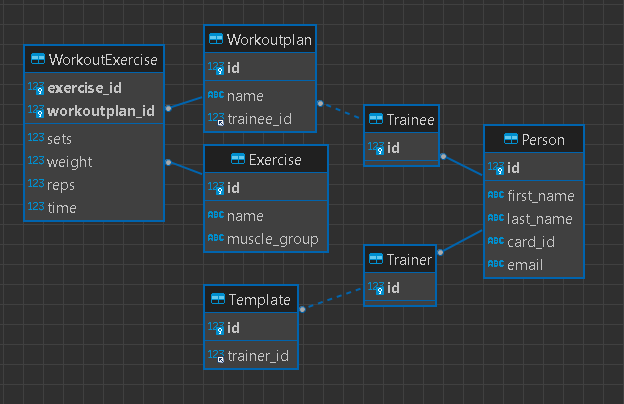
\includegraphics[width=1\textwidth]{pics/erd.png}
    \caption{ERD der Datenbankstruktur}
    \label{fig:erd}
\end{figure}
\newpage

\subsection{Datenbankverbindung für IntelliJ Projekt}
\begin{lstlisting}[language=Java,caption=Datenbank verbindung,label=lst:impl:foo]
    # Configuration file

    quarkus.swagger-ui.path=/swagger
    quarkus.swagger-ui.always-include=true
    
    # MS SQL DB connection
    quarkus.datasource.db-kind=mysql
    quarkus.datasource.username=****
    quarkus.datasource.password=***************
    quarkus.datasource.jdbc.url=jdbc:mysql://localhost:3306/AberGymDb
    #quarkus.hibernate-orm.database.generation=drop-and-create
    quarkus.hibernate-orm.database.generation=create
    #quarkus.hibernate-orm.database.generation=update
    #quarkus.hibernate-orm.sql-load-script=import.sql
\end{lstlisting}

Dieser Code zeigt die Konfigurationsdatei \cite{QuarkusHibernateORM} des Trainingsplan-Verwaltungssystems. Die Konfigurationsdatei legt die Einstellungen und Parameter fest, die das System beeinflussen. Die ersten beiden Einträge definieren den Pfad und die Verfügbarkeit der Swagger-UI, die eine grafische Benutzeroberfläche bietet, um das System zu testen und zu dokumentieren.
\newline
\newline
Die nächsten Einträge definieren die Verbindung zu einer MySQL-Datenbank. Der Befehl "quarkus.datasource.db-kind" gibt an, welcher Typ von Datenbank verwendet wird, in diesem Fall MySQL. "quarkus.datasource.username" und "quarkus.datasource.password" legen die Anmeldeinformationen für den Zugriff auf die Datenbank fest. "quarkus.datasource.jdbc.url" gibt die URL an, unter der die Datenbank erreichbar ist.
\newline
\newline
Der nächste Eintrag "quarkus.hibernate-orm.database.generation" gibt an, wie die Datenbank erstellt werden soll. In diesem Fall wird die Datenbank jedes Mal, wenn die Anwendung gestartet wird, erstellt, indem der Befehl "create" verwendet wird. Alternativ könnte der Befehl "update" verwendet werden, um die Datenbank zu aktualisieren, oder "drop-and-create", um die Datenbank vollständig zu löschen und neu zu erstellen.
\newline
\newline
Der letzte Eintrag "quarkus.hibernate-orm.sql-load-script" gibt an, welches SQL-Skript verwendet werden soll, um Daten in die Datenbank zu importieren. In diesem Fall wird kein Skript verwendet.
\newline
\newline
Die Konfigurationsdatei ist ein wichtiger Bestandteil des Trainingsplan-Verwaltungssystems, da sie die Verbindung zur Datenbank und die Erstellung der Datenbank definiert. Durch die Verwendung von Quarkus und Hibernate können Entwickler*innen schnell und einfach Datenbankanwendungen erstellen und konfigurieren.

\subsection{Demodaten für den Entwicklungsprozess der Mobile Anwendung}
\setauthor{Antonio Peric}  

Der Befehl "INSERT INTO" ist ein grundlegender SQL-Befehl \cite{SQLInsert}, der verwendet wird, um neue Datensätze in eine Datenbanktabelle einzufügen. Mit diesem Befehl können Daten in eine Tabelle eingefügt werden, indem der Befehl "VALUES" verwendet wird, um die Werte für die einzelnen Spalten anzugeben.
\newline
\newline
Die Syntax des Befehls "INSERT INTO" lautet wie folgt:

\begin{verbatim}
    INSERT INTO table_name (column1, column2, column3, ...)
    VALUES (value1, value2, value3, ...);
\end{verbatim}


Der Befehl beginnt mit dem Namen der Tabelle, in die die Daten eingefügt werden sollen. Anschließend werden in Klammern die Namen der Spalten angegeben, in die die Daten eingefügt werden sollen. Wenn der Befehl "INSERT INTO" verwendet wird, um in alle Spalten einer Tabelle einzufügen, kann die Angabe von Spaltennamen entfallen.
\newline
\newline
Die Werte, die in die Tabelle eingefügt werden sollen, werden nach dem Befehl "VALUES" aufgelistet und durch Kommas getrennt. Die Reihenfolge der Werte muss mit der Reihenfolge der Spaltennamen übereinstimmen.
\newline
\newline
Ein Beispiel für die Verwendung des Befehls "INSERT INTO" lautet wie folgt:
\begin{verbatim}
    INSERT INTO customers (name, address, city, state, zip)
    VALUES ('Max Mustermann', 'Musterstraße 1', 'Musterstadt', 'Musterland', '12345');
\end{verbatim}


In diesem Beispiel wird ein neuer Datensatz in die Tabelle "customers" eingefügt. Der Datensatz enthält die Werte "Max Mustermann" für den Namen, "Musterstraße 1" für die Adresse, "Musterstadt" für die Stadt, "Musterland" für den Staat und "12345" für die Postleitzahl.
\newline
\newline
Der Befehl "INSERT INTO" ist ein wichtiger Bestandteil der Datenmanipulation in SQL und wird häufig in Kombination mit anderen Befehlen wie "SELECT", "UPDATE" und "DELETE" verwendet, um Daten in einer Datenbank zu verwalten.
\newpage

\subsection{Import Datei für die Demo Daten}

\begin{verbatim}
    --------------------------------------------------------
    --  First Customer | Test data
    --------------------------------------------------------
    Insert into Person (first_name,last_name,email,cardId) 
        values ('Antonio','Peric','test@gmail.com','**************');
    Insert into Trainee (id) values (1);
    
    --------------------------------------------------------
    --  First Workoutplan
    --------------------------------------------------------
    
    Insert into Workoutplan (name,trainee_id) 
        values ('Ganzkörper Workout', 1);
    
    --  Exercise
    
    Insert into Exercise (name) values ('Liegestütze');
    Insert into Exercise (name) values ('Bench Press');
    Insert into Exercise (name) values ('Cable Flys');
    Insert into Exercise (name) values ('Incline Dumbell press');
    Insert into Exercise (name) values ('Biceps Curls');
    Insert into Exercise (name) values ('Triceps Extension');
    Insert into Exercise (name) values ('Triceps Curls');
    Insert into Exercise (name) values ('Skullcrusher');
    
    -- WorkoutExercise
    
    Insert into WorkoutExercise (sets,weight,reps,workoutplan_id, exercise_id) 
        values (5,0.0,50,1,1);
    Insert into WorkoutExercise (sets,weight,reps,workoutplan_id, exercise_id) 
        values (3,100.0,6,1,2);
    Insert into WorkoutExercise (sets,weight,reps,workoutplan_id, exercise_id) 
        values (3,20.0,25,1,3);
    Insert into WorkoutExercise (sets,weight,reps,workoutplan_id, exercise_id) 
        values (3,32.5,15,1,4);
    Insert into WorkoutExercise (sets,weight,reps,workoutplan_id, exercise_id) 
        values (5,12.5,15,1,5);
    Insert into WorkoutExercise (sets,weight,reps,workoutplan_id, exercise_id) 
        values (5,80.5,20,1,6);
    Insert into WorkoutExercise (sets,weight,reps,workoutplan_id, exercise_id) 
        values (2,80.0,20,1,7);
    Insert into WorkoutExercise (sets,weight,reps,workoutplan_id, exercise_id) 
        values (4,30.0,20,1,8);
    
    --------------------------------------------------------
    --  Second Workoutplan
    --------------------------------------------------------
    
    Insert into Workoutplan (name,trainee_id) values ('Ganzkörper Workout', 1);
    
    -- WorkoutExercise
    
    Insert into WorkoutExercise (sets,weight,reps,workoutplan_id, exercise_id) 
        values (5,10,50,2,1);
    Insert into WorkoutExercise (sets,weight,reps,workoutplan_id, exercise_id) 
        values (3,100.0,6,2,2);
    Insert into WorkoutExercise (sets,weight,reps,workoutplan_id, exercise_id) 
        values (3,20.0,25,2,3);
    Insert into WorkoutExercise (sets,weight,reps,workoutplan_id, exercise_id) 
        values (3,32.5,15,2,4);
    Insert into WorkoutExercise (sets,weight,reps,workoutplan_id, exercise_id) 
        values (5,12.5,15,2,5);
    Insert into WorkoutExercise (sets,weight,reps,workoutplan_id, exercise_id) 
        values (5,80.5,20,2,6);
    Insert into WorkoutExercise (sets,weight,reps,workoutplan_id, exercise_id) 
        values (2,80.0,20,2,7);
    Insert into WorkoutExercise (sets,weight,reps,workoutplan_id, exercise_id) 
        values (4,30.0,20,2,8);
\end{verbatim}
\newpage
Der bereitgestellte Code enthält SQL-Anweisungen, die in eine MySQL-Datenbank eingefügt werden sollen. Der erste Teil des Codes bezieht sich auf die Testdaten des ersten Kunden*inn und besteht aus zwei Insert-Anweisungen, die Daten in die Tabellen Person und Trainee einfügen.
\newline
\newline
Der zweite Teil des Codes bezieht sich auf den ersten Trainingsplan, der erstellt wird. Die Insert-Anweisung fügt einen neuen Eintrag in die Workoutplan-Tabelle ein und weist ihn dem Trainee mit der ID 1 zu.
\newline
\newline
Der dritte Teil des Codes bezieht sich auf die einzelnen Übungen, die Teil des Trainingsplans sind. Die Insert-Anweisungen fügen neue Einträge in die Exercise-Tabelle ein.
\newline
\newline
Der letzte Teil des Codes fügt die einzelnen Übungen mit den entsprechenden Sets, Gewichten und Wiederholungen in die WorkoutExercise-Tabelle ein und weist sie dem ersten Trainingsplan zu. Es werden auch Insert-Anweisungen für den zweiten Trainingsplan erstellt, die die gleichen Übungen wie der erste Trainingsplan enthalten, jedoch unterschiedliche Set-, Gewichts- und Wiederholungswerte aufweisen.
\newpage

\section{Integration des echten Backends}
\setauthor{Antonio Peric} 

\subsection{LeoCloud}
LeoCloud \cite{CanonicalApplication} ist ein Kubernetes Cluster \cite{KubernetesCluster}, der von der HTBLA Leonding betrieben wird und Schülern zur Verfügung steht. Kubernetes ist eine Container-Orchestrierungsplattform, die es Entwicklern ermöglicht, Containeranwendungen effizient zu erstellen, zu verwalten und zu skalieren. LeoCloud stellt Schülern eine Umgebung zur Verfügung, um praktische Erfahrungen mit der Container-Technologie und der Entwicklung von Cloud-Anwendungen zu sammeln.
\newline
\newline
Das Backend des Projekts AberGym-Syp wird auf LeoCloud gehostet, was den Entwicklern eine zuverlässige und skalierbare Plattform bietet, um die Anwendung bereitzustellen. Die Nutzung von Kubernetes ermöglicht eine automatisierte Skalierung von Ressourcen, die die Anforderungen der Anwendung erfüllen. So kann die Leistungsfähigkeit des Backends bei Bedarf erhöht werden, ohne manuelle Eingriffe von Seiten des Entwicklers.
\newline
\newline
Die Integration von Rest-Schnittstellen ermöglicht es, auf die Datenbank des Projekts AberGym-Syp zuzugreifen. Die MySql-Datenbank enthält alle relevanten Informationen, die von der Anwendung benötigt werden, um die Trainingspläne zu erstellen und zu verwalten. Das Einrichten von Rest-Schnittstellen erleichtert den Datenaustausch zwischen verschiedenen Anwendungen und ermöglicht eine einfache Integration in andere Systeme.
\newline
\newline
Die Nutzung von LeoCloud und Kubernetes ist ein Beispiel für den Einsatz moderner Cloud-Technologien in der Bildung. Es bietet Schülern eine Plattform, um praktische Erfahrungen mit den neuesten Technologien zu sammeln und ihre Fähigkeiten in der Entwicklung von Cloud-Anwendungen zu verbessern.


\begin{spacing}{1}
\chapter{Zusammenfassung}
\end{spacing}
Aufzählungen:

\begin{compactitem}
    \item Itemize Level 1
    \begin{compactitem}
        \item Itemize Level 2
        \begin{compactitem}
            \item Itemize Level 3 (vermeiden)
        \end{compactitem}
    \end{compactitem}
\end{compactitem}

\begin{compactenum}
    \item Enumerate Level 1
    \begin{compactenum}
        \item Enumerate Level 2
        \begin{compactenum}
            \item Enumerate Level 3 (vermeiden)
        \end{compactenum}
    \end{compactenum}
\end{compactenum}

\begin{compactdesc}
    \item[Desc] Level 1
    \begin{compactdesc}
        \item[Desc] Level 2 (vermeiden)
        \begin{compactdesc}
            \item[Desc] Level 3 (vermeiden)
        \end{compactdesc}
    \end{compactdesc}
\end{compactdesc}

\newpage
\pagenumbering{Roman}
\setcounter{page}{\value{RPages}}
\newacronym{guid}{GUID}{Globally Unique Identifier}
\newacronym{jit}{JIT}{Just In Time Compiler}
\newacronym{nfc}{NFC}{Near Field Communication}
\newacronym{rfid}{RFID}{Radio Frequency Identification}

% Usage:
% \gls{label} lowercase in text
% \Gls{label} Uppercase in text
% \newacronym{label}{abbrev}{full}
% \newglossaryentry{label}{settings}



%\setlength{\glsdescwidth}{0.8\linewidth}
\glsnogroupskiptrue
\printglossary[title=Glossar,toctitle=Glossar] %,style=long]
\spacing{1}{
%\bibliographystyle{IEEEtran}
\bibliographystyle{ieeetrande}
\bibliography{bib}
}
\listoffigures
\listoftables
\lstlistoflistings
\appendix
\addchap{Anhang}
\input{./sections/appendix}
\end{document}